\documentclass{article}
%%%%%%%%%%%%%%%%%%%%%%%%%%%%%%%%%%%%%%%%%%%%%%%%%%%%%%
% Math
%%%%%%%%%%%%%%%%%%%%%%%%%%%%%%%%%%%%%%%%%%%%%%%%%%%%%%
\usepackage{amsmath}
\usepackage{amssymb}
\usepackage{amsfonts} %para usar as fontes %matematicas, e pega fontes para \mathbb
\usepackage{amsthm}   %ambientes com teoremas (usar depois de amsmath)

%%%%%%%%%%%%%%%%%%%%%%%%%%%%%%%%%%%%%%%%%%%%%%%%%%%%%%
%Graphs
%%%%%%%%%%%%%%%%%%%%%%%%%%%%%%%%%%%%%%%%%%%%%%%%%%%%%%
\usepackage{graphics}
\usepackage{graphicx}
\usepackage{texdraw}
\usepackage{color}
\usepackage{subfigure} 
\usepackage{tikz}
\usepackage[usenames,dvipsnames]{pstricks}
\usepackage{epsfig}
\usepackage{pst-grad} % For gradients
\usepackage{pst-plot} % For axes
%\usepackage{movie15}
\usepackage{animate}
\usetikzlibrary{decorations.fractals}
\usepackage{tikz}
%\usepackage{wrapfig}
\usepackage{pstricks}
%%%%%%%%%%%%%%%%%%%%%%%%%%%%%%%%%%%%%%%%%%%%%%%%%%%%%%
% Format
%%%%%%%%%%%%%%%%%%%%%%%%%%%%%%%%%%%%%%%%%%%%%%%%%%%%%%
%\usepackage[figurename=Fig.]{caption}
\usepackage[labelformat=empty]{caption}
\usepackage{gensymb}
\usepackage{cancel}
\usepackage{caption} % removing prefix from figure caption in LaTeX
\usepackage{subcaption}
\usepackage{url}
\usepackage{setspace}
\usepackage{verbatim}
\usepackage{hyperref}
\usepackage{fancyhdr}
\usepackage{pgf}
%%%%%%%%%%%%%%%%%%%%%%%%%%%%%%%%%%%%%%%%%%%%%%%%%%%%%%
% Graphs path to the Picture Folder
%%%%%%%%%%%%%%%%%%%%%%%%%%%%%%%%%%%%%%%%%%%%%%%%%%%%%%
%\graphicspath{/home/henry/Desktop/UTEP_Proposal_Thesis/PhD_Thesis/Pictures}
\graphicspath{{Pictures/}{Data/}{References}} % Two folders Picture and Data   
%%%%%%%%%%%%%%%%%%%%%%%%%%%%%%%%%%%%%%%%%%%%%%%%%%%%%%
% page edition
%%%%%%%%%%%%%%%%%%%%%%%%%%%%%%%%%%%%%%%%%%%%%%%%%%%%%%
%\linespread{2.5}
\addtolength{\textwidth}{3cm}
\addtolength{\textheight}{3cm}
\addtolength{\hoffset}{-2cm}
% In case you need to adjust margins:
\topmargin=-0.5 in      %
\evensidemargin= .5 in     %
\oddsidemargin= .5 in      %
\textwidth = 7 in        %
\textheight = 9.0 in       %
\headsep = 0.15 in  
\pagestyle{fancyplain}
\lhead{\fancyplain{}{BLAST Performance using HTCondor}}
\rhead{\fancyplain{}{Henry R Moncada}}

%%%%%%%%%%%%%%%%%%%%%%%%%%%%%%%%%%%%%%%%%%%%%%%%%%%%%%
% bibliography
%%%%%%%%%%%%%%%%%%%%%%%%%%%%%%%%%%%%%%%%%%%%%%%%%%%%%%
%\usepackage{biblatex}
\bibliographystyle{plain}
%\bibliography{urlbib}

\begin{document}
% \centerline{\sc \large University of Texas at El Paso}
% \centerline{\sc \large Computational Science}
% \vspace{.5pc}
% \centerline{\sc \Large A short tutorial}
% \vspace{.5pc}
% \centerline{\sc \Large HTCondor - How to Submit jobs }
\title{University of Texas at El Paso\\
Summer Bioinformatics Project\\
BLAST Performance using HTCondor}
\vspace{.5pc}
\author{Henry R. Moncada}
\maketitle
\tableofcontents        % Generate Table of Contents

% On terminal to convert into html wed page
% pandoc HTCondor_submit.tex  -o test1.html
% pandoc -s  HTCondor_submit.tex  -o HTCondor_submit.html

%\vspace{2pc}
% \section*{References}
% Installions
% \footnotesize
% \begin{verbatim}
% http://www.installion.co.uk/ubuntu/trusty/universe/h/htcondor/install/index.html
% http://research.cs.wisc.edu/htcondor/manual/v7.9/3_2Installation.html
% \end{verbatim}
% \normalsize
% Downloads
% \footnotesize
% \begin{verbatim}
% http://research.cs.wisc.edu/htcondor/downloads/
% \end{verbatim}
% \normalsize
% Tutorials
% \footnotesize
% \begin{verbatim}
% https://research.cs.wisc.edu/htcondor/description.html
% http://research.cs.wisc.edu/htcondor/manual/quickstart.html
% https://research.cs.wisc.edu/htcondor/ubuntu/
% https://research.cs.wisc.edu/htcondor/tutorials/
% http://research.cs.wisc.edu/htcondor/manual/latest/12_Appendix_A.html
% \end{verbatim}
% \normalsize
% HTCondor into Python
% \footnotesize
% \begin{verbatim}
% https://research.cs.wisc.edu/htcondor/manual/v8.4/6_7Python_Bindings.html
% https://research.cs.wisc.edu/htcondor/HTCondorWeek2013/presentations/Bockelman_Python.pdf
% http://osgtech.blogspot.com/2014/03/submitting-jobs-to-htcondor-using-python.html
% https://github.com/candlerb/htcondor_dag.py
% \end{verbatim}
% \normalsize

\section{Introduction}
The following is a Bioinformatic project to speed up BLAST performance using HTcondor scheduler system. The project uses the following server computers to set up the pool computer available.
\begin{itemize}
 \item biolinuxXX sever
 \item cpslinuxXX sever
 \item apps sever
\end{itemize}

\section{HTCondor}
HTCondor is an open source job scheduler system develop by the University of Wisconsin that specialized in workload management for compute-intensive that supports High Throughput Computing (HTC). 
HTCondor provides a set of submission file commands that allow jobs to be submitted through various operating systems such as Linux, Unix, Mac OS, and Windows. It can be download. 
\footnotesize
\begin{verbatim}
https://research.cs.wisc.edu/htcondor/downloads/
\end{verbatim}
\normalsize
To work with HTCondor: 
\begin{itemize}
\item A pool of computers is provided to execute the job. 
\item HTCondor locates the computers that are available to run the job within the pool of computers. 
\item The pool of computers are divided into manager-execute (ME) and submit-execute (SE) computer.
\item HTCondor uses the ME computer to packages up the job and ships it off to the SE computers.
\item The SE computer runs the jobs and sends back  SE outputs to the ME computer. 
\end{itemize}

HTCondor is like other full-featured batch systems, HTCondor provides a job queueing mechanism, scheduling policy, priority scheme, resource monitoring, and resource management.
Users submit their serial or parallel jobs to HTCondor, HTCondor places them into a queue, chooses when and where to run the jobs based upon a policy, carefully monitors their progress, 
and ultimately informs the user upon completion\cite{HTcondor_What_is}.

\section{Install HTCondor}
To install HTcondor on Ubuntu LTS 12.04 and 14.04 we follow the instructions \cite{HTcondor_installation,HTcondor_installation_ubuntu}.
\begin{enumerate}
 \item Check that you have the correct repository enabled.  First, check that the universe repository is enabled by inspecting
 \verb+'/etc/apt/sources.list'+ with your favourite editor. You will need to use sudo to ensure that you have permissions to edit the file.
\begin{verbatim}
$ sudo gedit /etc/apt/sources.list
\end{verbatim}
\item If \textbf{universe} is not included on the \textbf{sources.list} file then modify the file on the following way so that it does.
  \begin{itemize}
    \item Ubuntu 12.04 LTS
    \begin{verbatim}
    deb http://us.archive.ubuntu.com/ubuntu/ precise universe
    \end{verbatim}
    \item Ubuntu 14.04 LTS
    \begin{verbatim}
    deb http://us.archive.ubuntu.com/ubuntu trusty main universe
    \end{verbatim}
  \end{itemize}
\item After any changes you should run this command to update your system.
\begin{verbatim}
$ sudo apt-get update
\end{verbatim}
You can now install the package like this.
\begin{verbatim}
$ sudo apt-get install htcondor
\end{verbatim}
Which will install htcondor and any other packages on which it depends.
\item Package Data
\begin{center}
\begin{tabular}{|l|l|} \hline
Package	& htcondor\\
Version	 & 8.0.5~dfsg.1-1ubuntu1 \\
Maintainer &	Ubuntu Developers <ubuntu-devel-discuss@lists.ubuntu.com>\\
Home page &	http://research.cs.wisc.edu/htcondor\\
Description &	distributed workload management system\\
Distro &	ubuntu\\
Release &	trusty\\
Repo &	universe\\
Section&	universe/science \\ \hline
\end{tabular}
\end{center}
\item Check if HTCondor is running 
\begin{verbatim}
$ ps -ef | grep condor
\end{verbatim}
Expected Result:
\begin{verbatim}
henry     5070 29934  0 16:53 pts/1    00:00:00 grep --color=auto condor
\end{verbatim}
\end{enumerate}

\section{Project}
\subsection{Login Procedure}
The login procedure is the same for each machine sever.
\begin{itemize}
\item Open a terminal
\item \textbf{Biolinux server:} Login into \verb+biolinuxXX+, we choose \verb+XX=20+.
\scriptsize\begin{verbatim}
henry@bluebottle:~/Desktop/TOOls/HT_Condor$ ssh hrmoncadalopez@biolinux20.bioinformatics.utep.edu

The authenticity of host 'biolinux09.bioinformatics.utep.edu (129.108.209.55)' can't be established.
ECDSA key fingerprint is 24:de:b9:89:e4:e9:76:9e:a5:e8:b2:b6:de:54:c7:f2.
Are you sure you want to continue connecting (yes/no)? yes
Warning: Permanently added 'biolinux09.bioinformatics.utep.edu,129.108.209.55' (ECDSA) to the list of known hosts.

###############################################################
#           Welcome to the Bioinformatics Network             #
#         All connections are monitored and recorded          #
#   Disconnect IMMEDIATELY if you are not an authorized user! #
###############################################################

hrmoncadalopez@biolinux09.bioinformatics.utep.edu's password: 

=============================================================================

       Use of computer and network facilities owned or operated by
    The University of Texas at El Paso requires prior authorization.
    Unauthorized access is prohibited.  Usage may be subject to
    security testing and monitoring, and affords no privacy
    guarantees, or expectations except as otherwise provided by
    applicable privacy laws.  Abuse is subject to criminal prosecution.
    Use of these facilities implies agreement to comply with the policy
    of The University of Texas at EL Paso.

=============================================================================
-bash-4.2$ 
\end{verbatim}
\normalsize
\item In a similar way login into the others serves.
\item \textbf{CPSlinux Server:} Open a terminal and login into \verb+cpslinuxXX+, we choose \verb+XX=01+.
\scriptsize\begin{verbatim}
henry@bluebottle:~/Desktop/TOOls/HT_Condor$ ssh hrmoncadalopez@cpslinux01.cps.utep.edu

-bash-4.2$ 
\end{verbatim}
\normalsize
\item \textbf{apps Server:} Open a terminal and login into \verb+apps+.
\scriptsize\begin{verbatim}
henry@bluebottle:~/Desktop/TOOls/HT_Condor/examples/split_sequence$ ssh hrmoncadalopez@apps.bioinformatics.utep.edu

-bash-4.2$ 
\end{verbatim}
\normalsize
\end{itemize}

\subsection{Check pool status}
\begin{itemize}
\item There are different HTCondor pull available. To check the number of cores availabale on each pull type the command \verb+condor_status+. 
\begin{enumerate}
\item biolinuxXX status
\scriptsize\begin{verbatim}
-bash-4.2$ condor_status
Name               OpSys      Arch   State     Activity LoadAv Mem   ActvtyTime

slot1@biolinux20.b LINUX      X86_64 Unclaimed Idle      0.000 1925  3+16:35:48
slot2@biolinux20.b LINUX      X86_64 Unclaimed Idle      0.000 1925  3+16:35:49
slot3@biolinux20.b LINUX      X86_64 Unclaimed Idle      0.000 1925  3+16:35:50
slot4@biolinux20.b LINUX      X86_64 Unclaimed Idle      0.000 1925  3+16:35:51
slot1@biolinux21.b LINUX      X86_64 Unclaimed Idle      0.000 1925  3+16:30:47
slot2@biolinux21.b LINUX      X86_64 Unclaimed Idle      0.000 1925  3+16:30:48
slot3@biolinux21.b LINUX      X86_64 Unclaimed Idle      0.000 1925  3+16:30:49
slot4@biolinux21.b LINUX      X86_64 Unclaimed Idle      0.000 1925  3+16:30:50
     Total Owner Claimed Unclaimed Matched Preempting Backfill

X86_64/LINUX     8     0       0         8       0          0        0

       Total     8     0       0         8       0          0        0
\end{verbatim}
\normalsize
\item cpslinuxXX status
\tiny\begin{verbatim}
-bash-4.2$ condor_status
\end{verbatim}
\normalsize
\item apps status
\scriptsize\begin{verbatim}
-bash-4.2$ condor_status
Name               OpSys      Arch   State     Activity LoadAv Mem   ActvtyTime

slot10@apps.bioinf LINUX      X86_64 Unclaimed Idle      0.000 5351  0+15:52:14
slot11@apps.bioinf LINUX      X86_64 Unclaimed Idle      0.000 5351  0+15:54:30
slot12@apps.bioinf LINUX      X86_64 Unclaimed Idle      0.000 5351  0+15:51:57
slot1@apps.bioinfo LINUX      X86_64 Unclaimed Idle      0.000 5351  0+15:54:24
slot2@apps.bioinfo LINUX      X86_64 Unclaimed Idle      0.000 5351  0+15:53:05
slot3@apps.bioinfo LINUX      X86_64 Unclaimed Idle      0.090 5351  0+15:54:36
slot4@apps.bioinfo LINUX      X86_64 Unclaimed Idle      0.000 5351  0+15:48:32
slot5@apps.bioinfo LINUX      X86_64 Unclaimed Idle      0.000 5351  0+15:50:04
slot6@apps.bioinfo LINUX      X86_64 Unclaimed Idle      0.000 5351  0+15:51:29
slot7@apps.bioinfo LINUX      X86_64 Unclaimed Idle      0.000 5351  0+15:53:36
slot8@apps.bioinfo LINUX      X86_64 Unclaimed Idle      0.000 5351  0+15:48:02
slot9@apps.bioinfo LINUX      X86_64 Unclaimed Idle      0.000 5351  0+15:52:35
slot1@biolinux07.b LINUX      X86_64 Unclaimed Idle      0.000 3949  0+15:50:29
slot2@biolinux07.b LINUX      X86_64 Unclaimed Idle      0.000 3949  0+15:52:30
slot3@biolinux07.b LINUX      X86_64 Unclaimed Idle      0.000 3949  0+15:54:40
slot4@biolinux07.b LINUX      X86_64 Unclaimed Idle      0.000 3949  0+15:54:05
                     Total Owner Claimed Unclaimed Matched Preempting Backfill

        X86_64/LINUX    16     0       0        16       0          0        0

               Total    16     0       0        16       0          0        0
\end{verbatim}
\normalsize
 \item 
\end{enumerate}
\end{itemize}
\section{Submition Example}
%Use the submit file template to submitting jobs to the central manager so they get distributed accordingly.
\subsection{Example program 1:}  \verb+Add_num.c+ is a C serial code that add number, like $1 + 2 = 3$
\begin{enumerate}
\item Program C-script :
\scriptsize\begin{verbatim}
      -bash-4.2$ vi Add_num.c

      #include <stdio.h>
      #include <stdlib.h>

      /* Define function to add two numbers */
      double add(double v1, double v2) {
      return v1 + v2;
      }

      int main (int argc, char *argv[]) {
      double a,b;

      /* read two numbers as command line arguments */
      if ( argc != 3 ) {
	printf("usage: %s num1 num2 \n", argv[0] );
	return (1);
      }

      a = b = 0;
      a = atof(argv[1]);
      b = atof(argv[2]);

      /* print their sum to standard output */
      printf("%g + %g = %g \n",a,b, add(a,b));
      return (0);
      }
\end{verbatim}
\normalsize
\item Compile and execute program:
\scriptsize\begin{verbatim}
-bash-4.2$ gcc Add_Num.c -o Add_Num

-bash-4.2$ ./Add_Num 1 2
1 + 2 = 3 
\end{verbatim}
\normalsize
\item Submittion job script: \verb+submit_Add_num+
\scriptsize\begin{verbatim}
-bash-4.2$ vi submit_Add_Num

Executable = /export/home/hrmoncadalopez/Desktop/HTCondor_examples/Add_Num
Arguments  = 1 2
Universe   = vanilla
Priority   = high
Should_transfer_files = No
#when_to_tranfer_output = ON_EXIT
Error      = /export/home/hrmoncadalopez/Desktop/HTCondor_examples/Add_Num.err
Output     = /export/home/hrmoncadalopez/Desktop/HTCondor_examples/Add_Num.out
Log        = /export/home/hrmoncadalopez/Desktop/HTCondor_examples/Add_Num.log
Queue
\end{verbatim}
\normalsize
\item  Submition job commands description:
\begin{itemize}
\item Executable: Name and location of your program
\item Arguments: The arguments you want to give to the execute. Same arguments execute with gcc.
\item Universe: The vanilla universe means a plain old job.
\item Priority: Set Priority high to allow the system to wake up computers
\item \verb+Should_transfer_files = No+
\item \verb+when_to_tranfer_output = ON_EXIT+
\item Error: Where Condor should put the standard error from your job. Our job isn't likely to have any, but we'll put it there to be safe
\item Output: Where Condor should put the standard output from your job.
\item Log: This is the name of a file where Condor will record information about your job's execution. While it's not required, it is a really good idea to have a log.
\item Queue : Tell Condor to submit this job
\end{itemize}
\item Submitte job to the central manager to get distributed accordingly:
\begin{itemize}
\item Submition Error:  If the central manager is not working \verb+biolinux09+, log-out from it and long-in into \verb+biolinux20+  or  \verb+biolinux21+. 
\scriptsize\begin{verbatim}
-bash-4.2$ condor_submit submit_Add_Num 

ERROR: Can't find address of local schedd
-bash-4.2$ 
\end{verbatim}
\normalsize
\item Submition success:
\scriptsize\begin{verbatim}
-bash-4.2$ condor_submit submit_Add_Num 

Submitting job(s).
1 job(s) submitted to cluster 11.
\end{verbatim}
\normalsize
\item Submition Results:
\scriptsize\begin{verbatim}
-rw-r--r--. 1 hrmoncadalopez student    0 Feb 10 12:09 Add_Num.err
-rw-r--r--. 1 hrmoncadalopez student 1015 Feb 10 12:09 Add_Num.log
-rw-r--r--. 1 hrmoncadalopez student   11 Feb 10 12:09 Add_Num.out
\end{verbatim}
\normalsize
\begin{itemize}
\item\verb+Add_Num.out+:
\scriptsize\begin{verbatim}
-bash-4.2$ vi Add_Num.1.out

  1 + 2 = 3
\end{verbatim}
\normalsize
\item \verb+Add_Num.log+:
\scriptsize\begin{verbatim}
-bash-4.2$ vi Add_Num.1.log

000 (010.001.000) 01/06 18:07:37 Job submitted from host: <129.108.209.63:64031?addrs=129.108.209.63-64031>
...
001 (010.001.000) 01/06 18:07:37 Job executing on host: <129.108.209.64:1644?addrs=129.108.209.64-1644>
...
006 (010.001.000) 01/06 18:07:37 Image size of job updated: 46012
0  -  MemoryUsage of job (MB)
0  -  ResidentSetSize of job (KB)
...
005 (010.001.000) 01/06 18:07:37 Job terminated.
(1) Normal termination (return value 0)
        Usr 0 00:00:00, Sys 0 00:00:00  -  Run Remote Usage
        Usr 0 00:00:00, Sys 0 00:00:00  -  Run Local Usage
        Usr 0 00:00:00, Sys 0 00:00:00  -  Total Remote Usage
        Usr 0 00:00:00, Sys 0 00:00:00  -  Total Local Usage
0  -  Run Bytes Sent By Job
0  -  Run Bytes Received By Job
0  -  Total Bytes Sent By Job
0  -  Total Bytes Received By Job
Partitionable Resources :    Usage  Request Allocated
   Cpus                 :                 1         1
   Disk (KB)            :       10       10  11071340
   Memory (MB)          :        0        1      1925
...

OUTPUT ERR:

-bash-4.2$ vi Add_Num.1.err
\end{verbatim}
\normalsize
\end{itemize}
\end{itemize}
\end{enumerate}

\subsection{Example program 2:}  \verb+submit_parameter_sweep.Add_Num+  is a HTcondor script that submit the previous C code into a pool of computers to be executed
\begin{enumerate}
\item Submittion sweep job script:
\scriptsize\begin{verbatim}
-bash-4.2$ vi submit_parameter_sweep.Add_Num 

Executable =  /export/home/hrmoncadalopez/Desktop/HTCondor_examples/Add_Num
Arguments  = 100 $(Process)
Universe   = vanilla
Priority   = high
Error      = /export/home/hrmoncadalopez/Desktop/HTCondor_examples/Add_Num.$(Process).err
Output     = /export/home/hrmoncadalopez/Desktop/HTCondor_examples/Add_Num.$(Process).out
Log        = /export/home/hrmoncadalopez/Desktop/HTCondor_examples/Add_Num.$(Process).log
#should_transfer_files = YES
Queue 10
\end{verbatim}
\normalsize
\item Submitte job to the central manager to get distributed accordingly:
\scriptsize\begin{verbatim}
-bash-4.2$ condor_submit submit_parameter_sweep.Add_Num 

Submitting job(s)..........
10 job(s) submitted to cluster 15.
\end{verbatim}
\normalsize
\item Submition Results:
\scriptsize\begin{verbatim}
-rw-r--r--. 1 hrmoncadalopez student    0 Feb 10 12:36 Add_Num.0.err
-rw-r--r--. 1 hrmoncadalopez student 1015 Feb 10 12:36 Add_Num.0.log
-rw-r--r--. 1 hrmoncadalopez student   15 Feb 10 12:36 Add_Num.0.out
-rw-r--r--. 1 hrmoncadalopez student    0 Feb 10 12:36 Add_Num.1.err
-rw-r--r--. 1 hrmoncadalopez student 1018 Feb 10 12:36 Add_Num.1.log
-rw-r--r--. 1 hrmoncadalopez student   15 Feb 10 12:36 Add_Num.1.out
-rw-r--r--. 1 hrmoncadalopez student    0 Feb 10 12:36 Add_Num.2.err
-rw-r--r--. 1 hrmoncadalopez student 1015 Feb 10 12:36 Add_Num.2.log
-rw-r--r--. 1 hrmoncadalopez student   15 Feb 10 12:36 Add_Num.2.out
-rw-r--r--. 1 hrmoncadalopez student    0 Feb 10 12:36 Add_Num.3.err
-rw-r--r--. 1 hrmoncadalopez student 1015 Feb 10 12:36 Add_Num.3.log
-rw-r--r--. 1 hrmoncadalopez student   15 Feb 10 12:36 Add_Num.3.out
-rw-r--r--. 1 hrmoncadalopez student    0 Feb 10 12:36 Add_Num.4.err
-rw-r--r--. 1 hrmoncadalopez student 1015 Feb 10 12:36 Add_Num.4.log
-rw-r--r--. 1 hrmoncadalopez student   15 Feb 10 12:36 Add_Num.4.out
-rw-r--r--. 1 hrmoncadalopez student    0 Feb 10 12:36 Add_Num.5.err
-rw-r--r--. 1 hrmoncadalopez st}udent 1015 Feb 10 12:36 Add_Num.5.log
-rw-r--r--. 1 hrmoncadalopez student   15 Feb 10 12:36 Add_Num.5.out
-rw-r--r--. 1 hrmoncadalopez student    0 Feb 10 12:36 Add_Num.6.err
-rw-r--r--. 1 hrmoncadalopez student 1015 Feb 10 12:36 Add_Num.6.log
-rw-r--r--. 1 hrmoncadalopez student   15 Feb 10 12:36 Add_Num.6.out
-rw-r--r--. 1 hrmoncadalopez student    0 Feb 10 12:36 Add_Num.7.err
-rw-r--r--. 1 hrmoncadalopez student 1018 Feb 10 12:36 Add_Num.7.log
-rw-r--r--. 1 hrmoncadalopez student   15 Feb 10 12:36 Add_Num.7.out
-rw-r--r--. 1 hrmoncadalopez student    0 Feb 10 12:36 Add_Num.8.err
-rw-r--r--. 1 hrmoncadalopez student 1015 Feb 10 12:36 Add_Num.8.log
-rw-r--r--. 1 hrmoncadalopez student   15 Feb 10 12:36 Add_Num.8.out
-rw-r--r--. 1 hrmoncadalopez student    0 Feb 10 12:36 Add_Num.9.err
-rw-r--r--. 1 hrmoncadalopez student 1018 Feb 10 12:36 Add_Num.9.log
-rw-r--r--. 1 hrmoncadalopez student   15 Feb 10 12:36 Add_Num.9.out
\end{verbatim}
\normalsize
\item OUTPUT OUT: \verb+Add_Num.1.out,  Add_Num.2.out ....+
\scriptsize\begin{verbatim}
-bash-4.2$ vi Add_Num.1.out

  100 + 1 = 101

-bash-4.2$ vi Add_Num.2.out

  100 + 2 = 102

.
.
.
\end{verbatim}
\normalsize
OUTPUT LOG: \verb+Add_Num.1.log,  Add_Num.2.log ....+
\scriptsize\begin{verbatim}
-bash-4.2$ vi Add_Num.1.log

000 (010.001.000) 01/06 18:07:37 Job submitted from host: <129.108.209.63:64031?addrs=129.108.209.63-64031>
...
001 (010.001.000) 01/06 18:07:37 Job executing on host: <129.108.209.64:1644?addrs=129.108.209.64-1644>
...
006 (010.001.000) 01/06 18:07:37 Image size of job updated: 46012
0  -  MemoryUsage of job (MB)
0  -  ResidentSetSize of job (KB)
...
005 (010.001.000) 01/06 18:07:37 Job terminated.
(1) Normal termination (return value 0)
        Usr 0 00:00:00, Sys 0 00:00:00  -  Run Remote Usage
        Usr 0 00:00:00, Sys 0 00:00:00  -  Run Local Usage
        Usr 0 00:00:00, Sys 0 00:00:00  -  Total Remote Usage
        Usr 0 00:00:00, Sys 0 00:00:00  -  Total Local Usage
0  -  Run Bytes Sent By Job
0  -  Run Bytes Received By Job
0  -  Total Bytes Sent By Job
0  -  Total Bytes Received By Job
Partitionable Resources :    Usage  Request Allocated
   Cpus                 :                 1         1
   Disk (KB)            :       10       10  11071340
   Memory (MB)          :        0        1      1925
...

OUTPUT ERR:

-bash-4.2$ vi Add_Num.1.err
\end{verbatim}
\normalsize
\end{enumerate}

\section{HTcondor with BLAST}
\subsection{BLAST: Submittion one single sequence}
\begin{itemize}
\item Sequence file
\scriptsize\begin{verbatim}
-bash-4.2$ vi sequence 

>test
MNYTLRTVSSSNITTIATTIISTILSRISTNKNNVTTPSTYENTTAISNYKTAYNITYYSDDYDDYEVNIVDIPHCDDGVYTT
\end{verbatim}
\normalsize
\item Submittion script - BLAST job
\scriptsize\begin{verbatim}
Universe   = vanilla
Executable = /applications/ncbi-blast-2.2.31+/bin/blastp
Arguments = -db /applications/blastDBs/uniref50 -query /export/home/hrmoncadalopez/Desktop/HTCondor_examples/sequence
Priority   = high
Should_transfer_files = No
#when_to_tranfer_output = ON_EXIT
Output = /export/home/hrmoncadalopez/Desktop/HTCondor_examples/blast.out
Error  = /export/home/hrmoncadalopez/Desktop/HTCondor_examples/blast.err
Log    = /export/home/hrmoncadalopez/Desktop/HTCondor_examples/blast.log
Queue
\end{verbatim}
\normalsize
\item Submitte BLAST job to the central manager to get distributed accordingly:  \verb+blastp_submit2+
\scriptsize\begin{verbatim}
-bash-4.2$ condor_submit blastp_submit2
Submitting job(s).
1 job(s) submitted to cluster 40
\end{verbatim}
\normalsize
\item Checking status process
\scriptsize\begin{verbatim}
-bash-4.2$ condor_status
Name               OpSys      Arch   State     Activity LoadAv Mem   ActvtyTime

slot1@biolinux20.b LINUX      X86_64 Claimed   Busy      0.170 1925  0+00:03:50       <=== one process is busy
slot2@biolinux20.b LINUX      X86_64 Unclaimed Idle      0.810 1925  0+00:10:42
slot3@biolinux20.b LINUX      X86_64 Unclaimed Idle      0.000 1925  0+00:10:43
slot4@biolinux20.b LINUX      X86_64 Unclaimed Idle      0.000 1925  0+00:10:44
slot1@biolinux21.b LINUX      X86_64 Unclaimed Idle      0.000 1925  0+00:12:35
slot2@biolinux21.b LINUX      X86_64 Unclaimed Idle      0.000 1925  0+00:12:36
slot3@biolinux21.b LINUX      X86_64 Unclaimed Idle      0.000 1925  0+00:12:37
slot4@biolinux21.b LINUX      X86_64 Unclaimed Idle      0.000 1925  0+00:12:38
                     Total Owner Claimed Unclaimed Matched Preempting Backfill
 
\end{verbatim}
\normalsize
\item Check output
\tiny\begin{verbatim}
V-bash-4.2$ vi blast.out

BLASTP 2.2.31+

Reference: Stephen F. Altschul, Thomas L. Madden, Alejandro A.
Schaffer, Jinghui Zhang, Zheng Zhang, Webb Miller, and David J.
Lipman (1997), "Gapped BLAST and PSI-BLAST: a new generation of
protein database search programs", Nucleic Acids Res. 25:3389-3402.

Reference for composition-based statistics: Alejandro A. Schaffer,
L. Aravind, Thomas L. Madden, Sergei Shavirin, John L. Spouge, Yuri
I. Wolf, Eugene V. Koonin, and Stephen F. Altschul (2001),
"Improving the accuracy of PSI-BLAST protein database searches with
composition-based statistics and other refinements", Nucleic Acids
Res. 29:2994-3005.
Database: uniref50.fasta
           15,065,016 sequences; 4,485,068,859 total letters
Query= test

Length=83
                                                                      Score     E
Sequences producing significant alignments:                          (Bits)  Value

UniRef50_Q86917  G-protein coupled receptor homolog Q2/3L n=82 Ta...  72.0    2e-13
UniRef50_A0A0F6QME8  G-protein-coupled chemokine receptor (Fragme...  55.5    2e-08
UniRef50_A0A0F9EU05  Uncharacterized protein (Fragment) n=1 Tax=m...  33.1    2.3
UniRef50_A0A0D8FR92  Resuscitation-promoting factor Rpf n=2 Tax=F...  33.1    4.2
UniRef50_B1L0P1  Uncharacterized protein n=1 Tax=Clostridium botu...  31.2    7.8
UniRef50_K9Z2B6  Signal peptidase I n=11 Tax=cellular organisms R...  31.6    9.1

>UniRef50_Q86917 G-protein coupled receptor homolog Q2/3L n=82 Tax=Capripoxvirus
RepID=VQ3L_SHEVK
Length=381

 Score = 72.0 bits (175),  Expect = 2e-13, Method: Compositional matrix adjust.
 Identities = 75/90 (83%), Positives = 77/90 (86%), Gaps = 7/90 (8%)

Query  1   MNYTLRTVSS-------SNITTIATTIISTILSRISTNKNNVTTPSTYENTTAISNYKTA  53
           MNYTL TVSS       SNITTIATTIISTILS ISTN+NNVTTPSTYENTT ISNY TA
Sbjct  1   MNYTLSTVSSATMYNSSSNITTIATTIISTILSTISTNQNNVTTPSTYENTTTISNYTTA  60

Query  54  YNITYYSDDYDDYEVNIVDIPHCDDGVYTT  83
           YN TYYSDDYDDYEV+IVDIPHCDDGV TT
Sbjct  61  YNTTYYSDDYDDYEVSIVDIPHCDDGVDTT  90

>UniRef50_A0A0F6QME8 G-protein-coupled chemokine receptor (Fragment) n=2 Tax=Lumpy
skin disease virus RepID=A0A0F6QME8_LSDV
Length=186

 Score = 55.5 bits (132),  Expect = 2e-08, Method: Compositional matrix adjust.
 Identities = 46/52 (88%), Positives = 48/52 (92%), Gaps = 0/52 (0%)

Query  32  KNNVTTPSTYENTTAISNYKTAYNITYYSDDYDDYEVNIVDIPHCDDGVYTT  83
           +NNVTTPSTYENTT ISNY TAYN TYYSDDYDDYEV+IVDIPHCDDGV TT
Sbjct  31  QNNVTTPSTYENTTTISNYTTAYNTTYYSDDYDDYEVSIVDIPHCDDGVDTT  82

>UniRef50_A0A0F9EU05 Uncharacterized protein (Fragment) n=1 Tax=marine sediment metagenome
RepID=A0A0F9EU05_9ZZZZ
Length=130

 Score = 33.1 bits (74),  Expect = 2.3, Method: Compositional matrix adjust.
 Identities = 25/81 (31%), Positives = 41/81 (51%), Gaps = 9/81 (11%)

Query  2   NYTLRTVSSSNITTIATTII--STILSRISTNKNNVTTPSTYENTTAIS--NYKTAYNIT  57
           N  L   S S  TT+A +++    ++SR    K  V   +T  +   I   N ++ Y+
Sbjct  11  NIALLGNSGSGKTTLAESMLMEGGVISR----KGEVDQKTTASDFREIEQENQRSIYSSV  66

Query  58  YYSDDYDDYEVNIVDIPHCDD  78
            Y++ Y D +VNI+D+P  DD
Sbjct  67  LYTE-YGDKKVNILDVPGADD  86

>UniRef50_A0A0D8FR92 Resuscitation-promoting factor Rpf n=2 Tax=Ferrimicrobium RepID=A0A0D8FR92_9ACTN
Length=364
Score = 33.1 bits (74),  Expect = 4.2, Method: Composition-based stats.
 Identities = 16/35 (46%), Positives = 23/35 (66%), Gaps = 2/35 (6%)

Query  22   STILSRISTNKNNVTTPSTYENTTA--ISNYKTAY  54
            S ++  ++TN+NNV T STYEN  +  + N  TAY
Sbjct  114  SAVIDALNTNQNNVATQSTYENVASGYVVNVITAY  148

>UniRef50_B1L0P1 Uncharacterized protein n=1 Tax=Clostridium botulinum (strain
Loch Maree / Type A3) RepID=B1L0P1_CLOBM
Length=100

 Score = 31.2 bits (69),  Expect = 7.8, Method: Compositional matrix adjust.
 Identities = 21/73 (29%), Positives = 32/73 (44%), Gaps = 4/73 (5%)

Query  6   RTVSSSNITTIATTIISTILSRISTNKNNVTTPSTYENTTAISNYKTAYNITYYSDDYDD  65
           R  S SN+ T+    +   + RI   KN     S  E TT  +N+K  YN     D ++D
Sbjct  18  RRGSVSNVYTLLKKKVQQSIDRIKQAKNG----SKEEKTTKKTNHKNNYNDKPKIDKFND  73

Query  66  YEVNIVDIPHCDD  78
           ++    D    +D
Sbjct  74  FDQRNYDFEKLED  86

>UniRef50_K9Z2B6 Signal peptidase I n=11 Tax=cellular organisms RepID=K9Z2B6_CYAAP
Length=187

 Score = 31.6 bits (70),  Expect = 9.1, Method: Compositional matrix adjust.
 Identities = 20/60 (33%), Positives = 29/60 (48%), Gaps = 4/60 (7%)

Query  2   NYTLRTVSSSNITTIATTIISTILSRISTNKNNVTTPSTYENTTAISNY----KTAYNIT  57
           N++LRT+   N TTIA  +I  +L RI   +       +   T AI +     K +YN T
Sbjct  11  NFSLRTIIKENFTTIAFGLILALLIRIFIAEPRFIPSESMYPTLAIGDRLVVDKVSYNFT  70

Lambda      K        H        a         alpha
   0.310    0.124    0.345    0.792     4.96

Gapped
Lambda      K        H        a         alpha    sigma
   0.267   0.0410    0.140     1.90     42.6     43.6

Effective search space used: 110598690330


  Database: uniref50.fasta
    Posted date:  Oct 8, 2015  12:47 PM
  Number of letters in database: 4,485,068,859
  Number of sequences in database:  15,065,016

Matrix: BLOSUM62
Gap Penalties: Existence: 11, Extension: 1
Neighboring words threshold: 11
Window for multiple hits: 40                                                         
                                                                                        141,1         Bot
\end{verbatim}
\normalsize
\end{itemize}
\subsection{Multiple BLAST submittions}
\begin{itemize}
\item Data Folder (\verb+Contig_Subsets_Translated+): DNA sequence files (Large data files)
\scriptsize\begin{verbatim}
-bash-4.2$ cd Contig_Subsets_Translated/
-bash-4.2$ ll
total 11176
-rw-r--r--. 1 hrmoncadalopez student 1515126 Feb 24 17:33 ContigSubset1TRANS.txt
-rw-r--r--. 1 hrmoncadalopez student 5408958 Feb 24 17:33 ContigSubset2TRANS.txt
-rw-r--r--. 1 hrmoncadalopez student 3194851 Feb 24 17:33 ContigSubset3TRANS.txt
-rw-r--r--. 1 hrmoncadalopez student  980511 Feb 24 17:33 ContigSubset4TRANS.txt
-rw-r--r--. 1 hrmoncadalopez student  239669 Feb 24 17:33 ContigSubset5TRANS.txt
-rw-r--r--. 1 hrmoncadalopez student   96357 Feb 24 17:33 ContigSubset6TRANS.txt
\end{verbatim}
\normalsize
\item How to split the data - Python programs : 
\begin{description}
\item [1.] \verb+Split_Sequence.py+ : This program construct output file with one sequence on each output file.
\scriptsize\begin{verbatim}
 # Set output files
outputBase = 'OUTPUT/output_' # output_1.txt, output_2.txt, etc.

# Open the input file 
input = open('Contig_Subsets_Translated/ContigSubset5TRANS.txt', 'r')

# Set split label
id_label = ">contig"

at = 0  # initialize output file
dest = None
for lines in input:
   if id_label in lines:
        if dest: dest.close()
        dest = open(outputBase + str(at) + '.txt', 'w') # write info into a file
        at += 1         # Increment the counter  output file
   dest.write(lines)
print ("Number of OUTPUT files is %d" %(at))
\end{verbatim}
\normalsize
\item [2.] \verb+Split_Sequence_bigger_chucks.py+ : This program construct output file with $n$ sequences on each output file.
\scriptsize\begin{verbatim}.
\scriptsize\begin{verbatim}
splitLen = 2                  # number of lines per file, pick multiples of 2
outputBase = 'OUTPUT/output_' # output.1.txt, output.2.txt, etc.

# Open the input file 
input = open('Contig_Subsets_Translated/ContigSubset5TRANS.txt', 'r').read().split('\n')

at = 0   # initialize output file
for lines in range(0, len(input), splitLen):
# First, get the list slice
    outputData = input[lines:lines+splitLen]

# Now open the output file, join the new slice with newlines and write it out. Then close the file.
    output = open(outputBase + str(at) + '.txt', 'w') #  open a file to write info
    output.write('\n'.join(outputData)) # # writes a string str to the file
    output.close()   # closes the opened file. A closed file cannot be read or written any more.

# Increment the counter
    at += 1

print ("Number of OUTPUT files is %d" %(at))
\end{verbatim}
\normalsize
\end{description}
\item Execute the program
\begin{verbatim}
-bash-4.2$ python Split_Sequence.py 

Number of OUTPUT files is 557
\end{verbatim}
\item Split files will store on \verb+OUTPUT/+
\scriptsize\begin{verbatim}
-bash-4.2$ cd OUTPUT/
-bash-4.2$ ll
total 600
-rw-r--r--. 1 hrmoncadalopez student 1156 Mar 13 15:16 output_0.txt
.
.
.
-rw-r--r--. 1 hrmoncadalopez student  944 Mar 13 15:16 output_100.txt
-rw-r--r--. 1 hrmoncadalopez student  263 Mar 13 15:16 output_101.txt
-rw-r--r--. 1 hrmoncadalopez student  210 Mar 13 15:16 output_102.txt
-rw-r--r--. 1 hrmoncadalopez student  221 Mar 13 15:16 output_103.txt
-rw-r--r--. 1 hrmoncadalopez student  207 Mar 13 15:16 output_104.txt
.
.
\end{verbatim}
\normalsize
\end{itemize}
\subsection{Submittion 5 jobs}
\begin{itemize}
\item BLAST sweep submittion \verb+(blastp_submit2_sweep)+ : %HTCondor quick start guide
HTCondor offers the use of a macro that can uniquely name each run's input and output file names. The \verb+$(Process)+ macro causes substitution by the process ID from
the job identifier. The submit description file for this proposed solution uniquely names the files:
\scriptsize\begin{verbatim}
-bash-4.2$ vi blastp_submit2_sweep

Universe   = vanilla
Executable = /applications/ncbi-blast-2.2.31+/bin/blastp
Arguments = -db /applications/blastDBs/uniref50 -query /export/home/hrmoncadalopez/Desktop/HTCondor_examples/OUTPUT/output_$(Process).txt
Priority   = high
Should_transfer_files = No
#when_to_tranfer_output = ON_EXIT
ID     = $(Cluster)_$(Process)
FNAME  = blast_output
Output = /export/home/hrmoncadalopez/Desktop/HTCondor_examples/BLAST_OUTPUT/$(FNAME)_$(ID).out
Error  = /export/home/hrmoncadalopez/Desktop/HTCondor_examples/BLAST_OUTPUT/$(FNAME)_$(ID).err
Log    = /export/home/hrmoncadalopez/Desktop/HTCondor_examples/BLAST_OUTPUT/$(FNAME)_$(ID).log
Queue 5
\end{verbatim}
\normalsize
Change the last line of the given submit description file
\footnotesize
\begin{verbatim}
Queue   to   Queue 5
\end{verbatim}
\normalsize
\item Submition description:
\begin{itemize}
\item  \verb+$(Cluster)+ : A macro variable that contains the job number, if you don't use it, your output will always be in the same file, if you re-submit.
\item \verb+Queue 5+  : There are $5$ instances (subjobs) to be run with the same job number.
\item \verb+$(Process)+ : A macro variable, means that the output, error and log files will be named according to the process number of the subjob (instances).
Keeping track which subjob is running. 
\item The value of \verb+$(Process)+ will not be exposed directly to the job, so you need to pass this to the arguments of your script.
\item The $5$ instances (subjobs) of this job will have process ID values that run from $0$ to $4$. 
\begin{itemize}
\item The input files for process ID $0$ are \verb+output_0.txt+, the one for process ID $1$ will \verb+output_1.txt+, and so on, all the way to process ID $4$, which will be files \verb+output_4.txt+. 
\item Using this macro also for the output file naming of each of the $5$ jobs creates \verb+blast_output_0.txt+ for process ID $0$, \verb+blast_output_1.txt+ for process ID $1$, and so on, to \verb+blast_output_4.txt+ for process ID $4$.
\end{itemize}
\end{itemize}
\item Check Status
\scriptsize  12.5   hrmoncadalopez  6/14 14:16   0+00:03:07 R  0   31.7 blastp -db /applic
\begin{verbatim}
-bash-4.2$ condor_status
Name               OpSys      Arch   State     Activity LoadAv Mem   ActvtyTime

slot10@apps.bioinf LINUX      X86_64 Unclaimed Idle      0.000 5351  0+15:52:14
slot11@apps.bioinf LINUX      X86_64 Unclaimed Idle      0.000 5351  0+15:54:30
slot12@apps.bioinf LINUX      X86_64 Unclaimed Idle      0.000 5351  0+15:51:57
slot1@apps.bioinfo LINUX      X86_64 Unclaimed Idle      0.000 5351  0+15:54:24
slot2@apps.bioinfo LINUX      X86_64 Unclaimed Idle      0.000 5351  0+15:53:05
slot3@apps.bioinfo LINUX      X86_64 Unclaimed Idle      0.090 5351  0+15:54:36
slot4@apps.bioinfo LINUX      X86_64 Unclaimed Idle      0.000 5351  0+15:48:32
slot5@apps.bioinfo LINUX      X86_64 Unclaimed Idle      0.000 5351  0+15:50:04
slot6@apps.bioinfo LINUX      X86_64 Unclaimed Idle      0.000 5351  0+15:51:29
slot7@apps.bioinfo LINUX      X86_64 Unclaimed Idle      0.000 5351  0+15:53:36
slot8@apps.bioinfo LINUX      X86_64 Unclaimed Idle      0.000 5351  0+15:48:02
slot9@apps.bioinfo LINUX      X86_64 Unclaimed Idle      0.000 5351  0+15:52:35
slot1@biolinux07.b LINUX      X86_64 Unclaimed Idle      0.000 3949  0+15:50:29
slot2@biolinux07.b LINUX      X86_64 Unclaimed Idle      0.000 3949  0+15:52:30
slot3@biolinux07.b LINUX      X86_64 Unclaimed Idle      0.000 3949  0+15:54:40
slot4@biolinux07.b LINUX      X86_64 Unclaimed Idle      0.000 3949  0+15:54:05
                     Total Owner Claimed Unclaimed Matched Preempting Backfill

        X86_64/LINUX    16     0       0        16       0          0        0

               Total    16     0       0        16       0          0        0
\end{verbatim}
\normalsize
\item Submit multiple jobs
\scriptsize
\begin{verbatim}
-bash-4.2$ condor_submit blastp_submit2_sweep 
Submitting job(s).....
5 job(s) submitted to cluster 8.
\end{verbatim}
Here: 
\begin{itemize}
 \item \verb+$(Cluster)+ job ID is equal to $8$ 
 \item \verb+$(Process)+ subjobs process ID values that run from $0$ to $4$. 
\end{itemize}
\normalsize
\item Check Status
\scriptsize
\begin{verbatim}              
-bash-4.2$ condor_status
Name               OpSys      Arch   State     Activity LoadAv Mem   ActvtyTime

slot10@apps.bioinf LINUX      X86_64 Unclaimed Idle      0.000 5351  0+15:57:14
slot11@apps.bioinf LINUX      X86_64 Unclaimed Idle      0.000 5351  0+15:59:30
slot12@apps.bioinf LINUX      X86_64 Unclaimed Idle      0.000 5351  0+15:56:57
slot1@apps.bioinfo LINUX      X86_64 Claimed   Busy      0.020 5351  0+00:00:18  <=== process is busy
slot2@apps.bioinfo LINUX      X86_64 Unclaimed Idle      0.000 5351  0+15:58:05
slot3@apps.bioinfo LINUX      X86_64 Unclaimed Idle      0.210 5351  0+15:59:36
slot4@apps.bioinfo LINUX      X86_64 Unclaimed Idle      0.000 5351  0+15:53:32
slot5@apps.bioinfo LINUX      X86_64 Unclaimed Idle      0.000 5351  0+15:55:04
slot6@apps.bioinfo LINUX      X86_64 Unclaimed Idle      0.000 5351  0+15:56:29
slot7@apps.bioinfo LINUX      X86_64 Unclaimed Idle      0.000 5351  0+15:58:36
slot8@apps.bioinfo LINUX      X86_64 Unclaimed Idle      0.000 5351  0+15:53:02
slot9@apps.bioinfo LINUX      X86_64 Unclaimed Idle      0.000 5351  0+15:57:35
slot1@biolinux07.b LINUX      X86_64 Claimed   Busy      0.000 3949  0+00:00:04  <=== process is busy
slot2@biolinux07.b LINUX      X86_64 Claimed   Busy      0.000 3949  0+00:00:05  <=== process is busy
slot3@biolinux07.b LINUX      X86_64 Claimed   Busy      0.320 3949  0+00:00:05  <=== process is busy
slot4@biolinux07.b LINUX      X86_64 Claimed   Busy      0.000 3949  0+00:00:06  <=== process is busy
                     Total Owner Claimed Unclaimed Matched Preempting Backfill

        X86_64/LINUX    16     0       5        11       0          0        0

               Total    16     0       5        11       0          0        0      
\end{verbatim}
\normalsize

\scriptsize
\begin{verbatim}
-bash-4.2$ condor_q

-- Schedd: apps.bioinformatics.utep.edu : <129.108.112.19:48332?...
 ID      OWNER            SUBMITTED     RUN_TIME ST PRI SIZE CMD               
   5.0   condor          5/31 21:01   0+00:00:01 H  0   0.0  RNAPredExec.pl CAG
   6.0   condor          5/31 21:01   0+00:00:01 H  0   0.0  RNAPredExec.pl CAG
   8.0   hrmoncadalopez  6/14 14:16   0+00:00:07 R  0   31.7 blastp -db /applic
   8.1   hrmoncadalopez  6/14 14:16   0+00:00:07 R  0   31.7 blastp -db /applic
   8.2   hrmoncadalopez  6/14 14:16   0+00:00:07 R  0   31.7 blastp -db /applic
   8.3   hrmoncadalopez  6/14 14:16   0+00:00:07 R  0   31.7 blastp -db /applic
   8.4   hrmoncadalopez  6/14 14:16   0+00:00:07 R  0   31.7 blastp -db /applic
7 jobs; 0 completed, 0 removed, 0 idle, 5 running, 2 held, 0 suspended
\end{verbatim}
\normalsize
\item Results:
\scriptsize
\begin{verbatim}
-bash-4.2$ ll
-rw-r--r--. 1 hrmoncadalopez student    0 Jun 14 13:28 blast_output_8_0.err
-rw-r--r--. 1 hrmoncadalopez student  506 Jun 14 13:33 blast_output_8_0.log
-rw-r--r--. 1 hrmoncadalopez student   17 Jun 14 13:29 blast_output_8_0.out
-rw-r--r--. 1 hrmoncadalopez student    0 Jun 14 13:28 blast_output_8_1.err
-rw-r--r--. 1 hrmoncadalopez student  506 Jun 14 13:33 blast_output_8_1.log
-rw-r--r--. 1 hrmoncadalopez student   17 Jun 14 13:29 blast_output_8_1.out
-rw-r--r--. 1 hrmoncadalopez student    0 Jun 14 13:28 blast_output_8_2.err
-rw-r--r--. 1 hrmoncadalopez student  506 Jun 14 13:33 blast_output_8_2.log
-rw-r--r--. 1 hrmoncadalopez student   17 Jun 14 13:29 blast_output_8_2.out
-rw-r--r--. 1 hrmoncadalopez student    0 Jun 14 13:28 blast_output_8_3.err
-rw-r--r--. 1 hrmoncadalopez student  506 Jun 14 13:33 blast_output_8_3.log
-rw-r--r--. 1 hrmoncadalopez student   17 Jun 14 13:29 blast_output_8_3.out
-rw-r--r--. 1 hrmoncadalopez student    0 Jun 14 13:28 blast_output_8_4.err
-rw-r--r--. 1 hrmoncadalopez student 1162 Jun 14 13:30 blast_output_8_4.log
-rw-r--r--. 1 hrmoncadalopez student 5094 Jun 14 13:30 blast_output_8_4.out

\end{verbatim}
\normalsize
\end{itemize}
\subsection{Submittion 25 Jobs}
\begin{itemize}
\item BLAST sweep submittion \verb+(blastp_submit2_sweep)+ : %HTCondor quick start guide
HTCondor offers the use of a macro that can uniquely name each run's input and output file names. The \verb+$(Process)+ macro causes substitution by the process ID from
the job identifier. The submit description file for this proposed solution uniquely names the files:
\scriptsize\begin{verbatim}
-bash-4.2$ vi blastp_submit2_sweep

Universe   = vanilla
Executable = /applications/ncbi-blast-2.2.31+/bin/blastp
Arguments = -db /applications/blastDBs/uniref50 -query /export/home/hrmoncadalopez/Desktop/HTCondor_examples/OUTPUT/output_$(Process).txt
Priority   = high
Should_transfer_files = No
#when_to_tranfer_output = ON_EXIT
ID     = $(Cluster)_$(Process)
FNAME  = blast_output
Output = /export/home/hrmoncadalopez/Desktop/HTCondor_examples/BLAST_OUTPUT/$(FNAME)_$(ID).out
Error  = /export/home/hrmoncadalopez/Desktop/HTCondor_examples/BLAST_OUTPUT/$(FNAME)_$(ID).err
Log    = /export/home/hrmoncadalopez/Desktop/HTCondor_examples/BLAST_OUTPUT/$(FNAME)_$(ID).log
Queue 25
\end{verbatim}
\normalsize
Change the last line of the given submit description file
\scriptsize
\begin{verbatim}
Queue   to   Queue 25
\end{verbatim}
\normalsize
\item Submition:
\begin{itemize}
 \item The $25$ instances of this job will have process ID values that run from $0$ to $24$. 
 \item The input files for process ID $0$ are \verb+output_0.txt+, the one for process ID $1$ will \verb+output_1.txt+, and so on, all the way to process ID $24$, which will be files \verb+output_4.txt+.
 \item Using this macro also for the output file naming of each of the $25$ jobs creates \verb+blast_output_0.txt+  for process ID $0$, \verb+blast_output_1.txt+ for process ID $1$, and so on, to \verb+blast_output_24.txt+ for process ID $24$.
\end{itemize}
\scriptsize
\begin{verbatim}
-bash-4.2$ 
Submitting job(s).........................
25 job(s) submitted to cluster 12.
\end{verbatim}
\normalsize
Here: 
\begin{itemize}
 \item \verb+$(Cluster)+ job ID is equal to $12$ 
 \item \verb+$(Process)+ subjobs process ID values that run from $0$ to $24$. 
\end{itemize}
\normalsize
\item Check Status
\scriptsize
\begin{verbatim}
-bash-4.2$ condor_status

Name               OpSys      Arch   State     Activity LoadAv Mem   ActvtyTime

slot10@apps.bioinf LINUX      X86_64 Claimed   Busy      0.000 5351  0+00:00:04
slot11@apps.bioinf LINUX      X86_64 Claimed   Busy      0.920 5351  0+00:00:05
slot12@apps.bioinf LINUX      X86_64 Claimed   Busy      0.000 5351  0+00:00:06
slot1@apps.bioinfo LINUX      X86_64 Claimed   Busy      0.000 5351  0+00:00:04
slot2@apps.bioinfo LINUX      X86_64 Claimed   Busy      0.000 5351  0+00:00:05
slot3@apps.bioinfo LINUX      X86_64 Claimed   Busy      1.000 5351  0+00:00:06
slot4@apps.bioinfo LINUX      X86_64 Claimed   Busy      0.000 5351  0+00:00:07
slot5@apps.bioinfo LINUX      X86_64 Claimed   Busy      0.000 5351  0+00:00:08
slot6@apps.bioinfo LINUX      X86_64 Claimed   Busy      0.000 5351  0+00:00:09
slot7@apps.bioinfo LINUX      X86_64 Claimed   Busy      0.000 5351  0+00:00:11
slot8@apps.bioinfo LINUX      X86_64 Claimed   Busy      0.000 5351  0+00:00:03
slot9@apps.bioinfo LINUX      X86_64 Claimed   Busy      0.000 5351  0+00:00:04
slot1@biolinux07.b LINUX      X86_64 Claimed   Busy      0.000 3949  0+00:00:04
slot2@biolinux07.b LINUX      X86_64 Claimed   Busy      0.000 3949  0+00:00:05
slot3@biolinux07.b LINUX      X86_64 Claimed   Busy      0.500 3949  0+00:00:06
slot4@biolinux07.b LINUX      X86_64 Claimed   Busy      0.000 3949  0+00:00:07
                     Total Owner Claimed Unclaimed Matched Preempting Backfill

        X86_64/LINUX    16     0      16         0       0          0        0

               Total    16     0      16         0       0          0        0

\end{verbatim}
\normalsize
\item 
\scriptsize
\begin{verbatim}
-bash-4.2$ condor_q

-- Schedd: apps.bioinformatics.utep.edu : <129.108.112.19:48332?...
 ID      OWNER            SUBMITTED     RUN_TIME ST PRI SIZE CMD               
   5.0   condor          5/31 21:01   0+00:00:01 H  0   0.0  RNAPredExec.pl CAG
   6.0   condor          5/31 21:01   0+00:00:01 H  0   0.0  RNAPredExec.pl CAG
  12.0   hrmoncadalopez  6/14 14:16   0+00:03:07 R  0   31.7 blastp -db /applic
  12.1   hrmoncadalopez  6/14 14:16   0+00:03:07 R  0   31.7 blastp -db /applic
  12.2   hrmoncadalopez  6/14 14:16   0+00:03:07 R  0   31.7 blastp -db /applic
  12.3   hrmoncadalopez  6/14 14:16   0+00:03:07 R  0   31.7 blastp -db /applic
  12.5   hrmoncadalopez  6/14 14:16   0+00:03:07 R  0   31.7 blastp -db /applic
  12.10  hrmoncadalopez  6/14 14:16   0+00:03:07 R  0   31.7 blastp -db /applic
  12.15  hrmoncadalopez  6/14 14:16   0+00:03:07 R  0   31.7 blastp -db /applic
  12.16  hrmoncadalopez  6/14 14:16   0+00:01:08 R  0   31.7 blastp -db /applic
  12.17  hrmoncadalopez  6/14 14:16   0+00:01:08 R  0   31.7 blastp -db /applic
  12.18  hrmoncadalopez  6/14 14:16   0+00:01:03 R  0   31.7 blastp -db /applic
  12.19  hrmoncadalopez  6/14 14:16   0+00:01:03 R  0   31.7 blastp -db /applic
  12.20  hrmoncadalopez  6/14 14:16   0+00:00:37 R  0   31.7 blastp -db /applic
  12.21  hrmoncadalopez  6/14 14:16   0+00:00:36 R  0   31.7 blastp -db /applic
  12.22  hrmoncadalopez  6/14 14:16   0+00:00:32 R  0   31.7 blastp -db /applic
  12.23  hrmoncadalopez  6/14 14:16   0+00:00:25 R  0   31.7 blastp -db /applic
  12.24  hrmoncadalopez  6/14 14:16   0+00:00:22 R  0   31.7 blastp -db /applic

18 jobs; 0 completed, 0 removed, 0 idle, 16 running, 2 held, 0 suspended
\end{verbatim}
\normalsize
\item Results:
\scriptsize
\begin{verbatim}
    -bash-4.2$ cd BLAST_OUTPUT/

    -bash-4.2$ ll

    total 4260
    -rw-r--r--. 1 hrmoncadalopez student      0 Jun 14 14:16 blast_output_12_0.err
    -rw-r--r--. 1 hrmoncadalopez student   1317 Jun 14 14:24 blast_output_12_0.log
    -rw-r--r--. 1 hrmoncadalopez student 826969 Jun 14 14:24 blast_output_12_0.out
    -rw-r--r--. 1 hrmoncadalopez student      0 Jun 14 14:16 blast_output_12_10.err
    -rw-r--r--. 1 hrmoncadalopez student   1319 Jun 14 14:23 blast_output_12_10.log
    -rw-r--r--. 1 hrmoncadalopez student 826969 Jun 14 14:23 blast_output_12_10.out
    -rw-r--r--. 1 hrmoncadalopez student      0 Jun 14 14:16 blast_output_12_11.err
    -rw-r--r--. 1 hrmoncadalopez student   1168 Jun 14 14:19 blast_output_12_11.log
    -rw-r--r--. 1 hrmoncadalopez student   6148 Jun 14 14:19 blast_output_12_11.out
    -rw-r--r--. 1 hrmoncadalopez student      0 Jun 14 14:16 blast_output_12_12.err
    -rw-r--r--. 1 hrmoncadalopez student   1168 Jun 14 14:19 blast_output_12_12.log
    -rw-r--r--. 1 hrmoncadalopez student   2769 Jun 14 14:19 blast_output_12_12.out
    -rw-r--r--. 1 hrmoncadalopez student      0 Jun 14 14:16 blast_output_12_13.err
    -rw-r--r--. 1 hrmoncadalopez student   1168 Jun 14 14:19 blast_output_12_13.log
    -rw-r--r--. 1 hrmoncadalopez student   3536 Jun 14 14:19 blast_output_12_13.out
    -rw-r--r--. 1 hrmoncadalopez student      0 Jun 14 14:16 blast_output_12_14.err
    -rw-r--r--. 1 hrmoncadalopez student   1168 Jun 14 14:19 blast_output_12_14.log
    -rw-r--r--. 1 hrmoncadalopez student   5094 Jun 14 14:19 blast_output_12_14.out
    -rw-r--r--. 1 hrmoncadalopez student      0 Jun 14 14:16 blast_output_12_15.err
    -rw-r--r--. 1 hrmoncadalopez student   1315 Jun 14 14:23 blast_output_12_15.log
    -rw-r--r--. 1 hrmoncadalopez student 826969 Jun 14 14:23 blast_output_12_15.out
    -rw-r--r--. 1 hrmoncadalopez student      0 Jun 14 14:16 blast_output_12_16.err
    -rw-r--r--. 1 hrmoncadalopez student   1172 Jun 14 14:20 blast_output_12_16.log
    -rw-r--r--. 1 hrmoncadalopez student   6148 Jun 14 14:20 blast_output_12_16.out
    -rw-r--r--. 1 hrmoncadalopez student      0 Jun 14 14:17 blast_output_12_17.err
    -rw-r--r--. 1 hrmoncadalopez student   1172 Jun 14 14:21 blast_output_12_17.log
    -rw-r--r--. 1 hrmoncadalopez student   2769 Jun 14 14:21 blast_output_12_17.out
    -rw-r--r--. 1 hrmoncadalopez student      0 Jun 14 14:17 blast_output_12_18.err
    -rw-r--r--. 1 hrmoncadalopez student   1168 Jun 14 14:21 blast_output_12_18.log
    -rw-r--r--. 1 hrmoncadalopez student   3536 Jun 14 14:21 blast_output_12_18.out
    -rw-r--r--. 1 hrmoncadalopez student      0 Jun 14 14:17 blast_output_12_19.err
    -rw-r--r--. 1 hrmoncadalopez student   1162 Jun 14 14:21 blast_output_12_19.log
    -rw-r--r--. 1 hrmoncadalopez student   5094 Jun 14 14:21 blast_output_12_19.out
    -rw-r--r--. 1 hrmoncadalopez student      0 Jun 14 14:16 blast_output_12_1.err
    -rw-r--r--. 1 hrmoncadalopez student   1170 Jun 14 14:24 blast_output_12_1.log
    -rw-r--r--. 1 hrmoncadalopez student   6148 Jun 14 14:24 blast_output_12_1.out
    -rw-r--r--. 1 hrmoncadalopez student      0 Jun 14 14:17 blast_output_12_20.err
    -rw-r--r--. 1 hrmoncadalopez student   1319 Jun 14 14:25 blast_output_12_20.log
    -rw-r--r--. 1 hrmoncadalopez student 826969 Jun 14 14:25 blast_output_12_20.out
    -rw-r--r--. 1 hrmoncadalopez student      0 Jun 14 14:17 blast_output_12_21.err
    -rw-r--r--. 1 hrmoncadalopez student   1172 Jun 14 14:21 blast_output_12_21.log
    -rw-r--r--. 1 hrmoncadalopez student   6148 Jun 14 14:21 blast_output_12_21.out
    -rw-r--r--. 1 hrmoncadalopez student      0 Jun 14 14:17 blast_output_12_22.err
    -rw-r--r--. 1 hrmoncadalopez student   1172 Jun 14 14:22 blast_output_12_22.log
    -rw-r--r--. 1 hrmoncadalopez student   2769 Jun 14 14:22 blast_output_12_22.out
    -rw-r--r--. 1 hrmoncadalopez student      0 Jun 14 14:17 blast_output_12_23.err
    -rw-r--r--. 1 hrmoncadalopez student   1172 Jun 14 14:21 blast_output_12_23.log
    -rw-r--r--. 1 hrmoncadalopez student   3536 Jun 14 14:21 blast_output_12_23.out
    -rw-r--r--. 1 hrmoncadalopez student      0 Jun 14 14:17 blast_output_12_24.err
    -rw-r--r--. 1 hrmoncadalopez student   1168 Jun 14 14:22 blast_output_12_24.log
    -rw-r--r--. 1 hrmoncadalopez student   5094 Jun 14 14:22 blast_output_12_24.out
    -rw-r--r--. 1 hrmoncadalopez student      0 Jun 14 14:16 blast_output_12_2.err
    -rw-r--r--. 1 hrmoncadalopez student   1169 Jun 14 14:23 blast_output_12_2.log
    -rw-r--r--. 1 hrmoncadalopez student   2769 Jun 14 14:23 blast_output_12_2.out
    -rw-r--r--. 1 hrmoncadalopez student      0 Jun 14 14:16 blast_output_12_3.err
    -rw-r--r--. 1 hrmoncadalopez student   1166 Jun 14 14:23 blast_output_12_3.log
    -rw-r--r--. 1 hrmoncadalopez student   3536 Jun 14 14:23 blast_output_12_3.out
    -rw-r--r--. 1 hrmoncadalopez student      0 Jun 14 14:16 blast_output_12_4.err
    -rw-r--r--. 1 hrmoncadalopez student   1168 Jun 14 14:19 blast_output_12_4.log
    -rw-r--r--. 1 hrmoncadalopez student   5094 Jun 14 14:19 blast_output_12_4.out
    -rw-r--r--. 1 hrmoncadalopez student      0 Jun 14 14:16 blast_output_12_5.err
    -rw-r--r--. 1 hrmoncadalopez student   1319 Jun 14 14:23 blast_output_12_5.log
    -rw-r--r--. 1 hrmoncadalopez student 826969 Jun 14 14:23 blast_output_12_5.out
    -rw-r--r--. 1 hrmoncadalopez student      0 Jun 14 14:16 blast_output_12_6.err
    -rw-r--r--. 1 hrmoncadalopez student   1168 Jun 14 14:19 blast_output_12_6.log
    -rw-r--r--. 1 hrmoncadalopez student   6148 Jun 14 14:18 blast_output_12_6.out
    -rw-r--r--. 1 hrmoncadalopez student      0 Jun 14 14:16 blast_output_12_7.err
    -rw-r--r--. 1 hrmoncadalopez student   1168 Jun 14 14:19 blast_output_12_7.log
    -rw-r--r--. 1 hrmoncadalopez student   2769 Jun 14 14:19 blast_output_12_7.out
    -rw-r--r--. 1 hrmoncadalopez student      0 Jun 14 14:16 blast_output_12_8.err
    -rw-r--r--. 1 hrmoncadalopez student   1168 Jun 14 14:19 blast_output_12_8.log
    -rw-r--r--. 1 hrmoncadalopez student   3536 Jun 14 14:19 blast_output_12_8.out
    -rw-r--r--. 1 hrmoncadalopez student      0 Jun 14 14:16 blast_output_12_9.err
    -rw-r--r--. 1 hrmoncadalopez student   1168 Jun 14 14:19 blast_output_12_9.log
    -rw-r--r--. 1 hrmoncadalopez student   5094 Jun 14 14:19 blast_output_12_9.out
\end{verbatim}
\normalsize
\end{itemize}
\subsection{Measuring Queue Time and Execution Time on HTcondor}
To measured the computational execution time on Condor. We are going to use the \verb+condor_history+ to extract the time information need to estimate the execute time. 
\begin{itemize}
\item Synopsis: \verb+Condor_history+
\scriptsize
\begin{verbatim}
condor_history [-help]

condor_history [-name name] [-pool centralmanagerhostname[:portnumber]] [-backwards] [-forwards] [-constraint expr] [-file filename]
	  [-userlog filename] [-format formatString AttributeName] [-autoformat[:tn,lVh] attr1 [attr2 ...]] [-l | -long | -xml] 
	  [-match | -limit number] [cluster | cluster.process | owner]
\end{verbatim}
\normalsize
\item \verb+condor_history -help+
\scriptsize
\begin{verbatim}
    -bash-4.2$ condor_history -help
    
    Usage: condor_history [source] [restriction-list] [options]

      where [source] is one of
	    -file <file>		Read history data from specified file
	    -userlog <file>		Read job data specified userlog file
	    -name <schedd-name>	Remote schedd to read from
	    -pool <collector-name>	Pool remote schedd lives in.
      If neither -pool, -name, -userlog or -file is specified, then the local history file is used.

      and [restriction-list] is one or more of
	    <cluster>		Get information about specific cluster
	    <cluster>.<proc>	Get information about specific job
	    <owner>			Information about jobs owned by <owner>
	    -constraint <expr>	Information about jobs matching <expr>

      and [options] are one or more of
	    -help			Display this screen
	    -backwards		List jobs in reverse chronological order
	    -forwards		List jobs in chronological order
	    -limit <number>		Limit the number of jobs displayed
	    -match <number>		Old name for -limit
	    -long			Display entire classads
	    -wide[:<width>]	con	Don't truncate fields to fit into 80 columns
	    -format <fmt> <attr>	Display attr using printf formatting
	    -autoformat[:lhVr,tng] <attr> [<attr2 ...]   Display attr(s) with automatic formatting
	    -af[:lhVr,tng] <attr> [<attr2 ...]	    Same as -autoformat above
	    
		where the [lhVr,tng] options influence the automatic formatting:
		l	attribute labels
		h	attribute column headings
		V	%V formatting (string values are quoted)
		r	%r formatting (raw/unparsed values)
		t	tab before each value (default is space)
		g	newline between ClassAds, no space before values
		,	comma after each value
		n	newline after each value
		use -af:h to get tabular values with headings
	    -print-format <file>	Use <file> to specify the attributes and formatting
				    (experimental, see htcondor-wiki for more information)
    -bash-4.2$
\end{verbatim}
\normalsize
\item \verb+condor_history -limit number_of_events+
\tiny
\begin{verbatim}
    -bash-4.2$ condor_history -limit 10
    ID     OWNER          SUBMITTED   RUN_TIME     ST COMPLETED   CMD            
      12.20  hrmoncadalopez  6/14 14:16   0+00:06:05 C   6/14 14:25 /applications/ncbi-blast-2.2.31+/bin/blastp -db /applications/blastDBs/uniref50 -query /export/home/hrmonc
      12.0   hrmoncadalopez  6/14 14:16   0+00:07:58 C   6/14 14:24 /applications/ncbi-blast-2.2.31+/bin/blastp -db /applications/blastDBs/uniref50 -query /export/home/hrmonc
      12.1   hrmoncadalopez  6/14 14:16   0+00:07:21 C   6/14 14:24 /applications/ncbi-blast-2.2.31+/bin/blastp -db /applications/blastDBs/uniref50 -query /export/home/hrmonc
      12.15  hrmoncadalopez  6/14 14:16   0+00:06:54 C   6/14 14:23 /applications/ncbi-blast-2.2.31+/bin/blastp -db /applications/blastDBs/uniref50 -query /export/home/hrmonc
      12.5   hrmoncadalopez  6/14 14:16   0+00:06:53 C   6/14 14:23 /applications/ncbi-blast-2.2.31+/bin/blastp -db /applications/blastDBs/uniref50 -query /export/home/hrmonc
      12.2   hrmoncadalopez  6/14 14:16   0+00:06:49 C   6/14 14:23 /applications/ncbi-blast-2.2.31+/bin/blastp -db /applications/blastDBs/uniref50 -query /export/home/hrmonc
      12.10  hrmoncadalopez  6/14 14:16   0+00:06:49 C   6/14 14:23 /applications/ncbi-blast-2.2.31+/bin/blastp -db /applications/blastDBs/uniref50 -query /export/home/hrmonc
      12.3   hrmoncadalopez  6/14 14:16   0+00:06:33 C   6/14 14:23 /applications/ncbi-blast-2.2.31+/bin/blastp -db /applications/blastDBs/uniref50 -query /export/home/hrmonc
      12.22  hrmoncadalopez  6/14 14:16   0+00:02:28 C   6/14 14:22 /applications/ncbi-blast-2.2.31+/bin/blastp -db /applications/blastDBs/uniref50 -query /export/home/hrmonc
      12.24  hrmoncadalopez  6/14 14:16   0+00:02:17 C   6/14 14:22 /applications/ncbi-blast-2.2.31+/bin/blastp -db /applications/blastDBs/uniref50 -query /export/home/hrmonc
    -bash-4.2$ 
\end{verbatim}
\normalsize

\item \verb+condor_history -match number_of_events+
\tiny
\begin{verbatim}
    -bash-4.2$ condor_history -match 1
    ID     OWNER          SUBMITTED   RUN_TIME     ST COMPLETED   CMD            
      12.20  hrmoncadalopez  6/14 14:16   0+00:06:05 C   6/14 14:25 /applications/ncbi-blast-2.2.31+/bin/blastp -db /applications/blastDBs/uniref50 -query /export/home/hrmoncadalop
      
    -bash-4.2$ condor_history -match 2
    ID     OWNER          SUBMITTED   RUN_TIME     ST COMPLETED   CMD            
      12.20  hrmoncadalopez  6/14 14:16   0+00:06:05 C   6/14 14:25 /applications/ncbi-blast-2.2.31+/bin/blastp -db /applications/blastDBs/uniref50 -query /export/home/hrmoncadalop
      12.0   hrmoncadalopez  6/14 14:16   0+00:07:58 C   6/14 14:24 /applications/ncbi-blast-2.2.31+/bin/blastp -db /applications/blastDBs/uniref50 -query /export/home/hrmoncadalop
    -bash-4.2$ 
\end{verbatim}
\normalsize

\item \verb+condor_history ClusterId = +
\tiny
\begin{verbatim}
-bash-4.2$ condor_history ClusterId = 12
 ID     OWNER          SUBMITTED   RUN_TIME     ST COMPLETED   CMD            
  12.20  hrmoncadalopez  6/14 14:16   0+00:06:05 C   6/14 14:25 /applications/ncbi-blast-2.2.31+/bin/blastp -db /applications/blastDBs/uniref50 -query /export/home/hrmoncadalo
  12.0   hrmoncadalopez  6/14 14:16   0+00:07:58 C   6/14 14:24 /applications/ncbi-blast-2.2.31+/bin/blastp -db /applications/blastDBs/uniref50 -query /export/home/hrmoncadalo
  12.1   hrmoncadalopez  6/14 14:16   0+00:07:21 C   6/14 14:24 /applications/ncbi-blast-2.2.31+/bin/blastp -db /applications/blastDBs/uniref50 -query /export/home/hrmoncadalo
  12.15  hrmoncadalopez  6/14 14:16   0+00:06:54 C   6/14 14:23 /applications/ncbi-blast-2.2.31+/bin/blastp -db /applications/blastDBs/uniref50 -query /export/home/hrmoncadalo
  12.5   hrmoncadalopez  6/14 14:16   0+00:06:53 C   6/14 14:23 /applications/ncbi-blast-2.2.31+/bin/blastp -db /applications/blastDBs/uniref50 -query /export/home/hrmoncadalo
  12.2   hrmoncadalopez  6/14 14:16   0+00:06:49 C   6/14 14:23 /applications/ncbi-blast-2.2.31+/bin/blastp -db /applications/blastDBs/uniref50 -query /export/home/hrmoncadalo
  12.10  hrmoncadalopez  6/14 14:16   0+00:06:49 C   6/14 14:23 /applications/ncbi-blast-2.2.31+/bin/blastp -db /applications/blastDBs/uniref50 -query /export/home/hrmoncadalo
  12.3   hrmoncadalopez  6/14 14:16   0+00:06:33 C   6/14 14:23 /applications/ncbi-blast-2.2.31+/bin/blastp -db /applications/blastDBs/uniref50 -query /export/home/hrmoncadalo
  12.22  hrmoncadalopez  6/14 14:16   0+00:02:28 C   6/14 14:22 /applications/ncbi-blast-2.2.31+/bin/blastp -db /applications/blastDBs/uniref50 -query /export/home/hrmoncadalo
  12.24  hrmoncadalopez  6/14 14:16   0+00:02:17 C   6/14 14:22 /applications/ncbi-blast-2.2.31+/bin/blastp -db /applications/blastDBs/uniref50 -query /export/home/hrmoncadalo
  12.23  hrmoncadalopez  6/14 14:16   0+00:02:07 C   6/14 14:21 /applications/ncbi-blast-2.2.31+/bin/blastp -db /applications/blastDBs/uniref50 -query /export/home/hrmoncadalo
  12.17  hrmoncadalopez  6/14 14:16   0+00:02:39 C   6/14 14:21 /applications/ncbi-blast-2.2.31+/bin/blastp -db /applications/blastDBs/uniref50 -query /export/home/hrmoncadalo
  12.21  hrmoncadalopez  6/14 14:16   0+00:01:58 C   6/14 14:21 /applications/ncbi-blast-2.2.31+/bin/blastp -db /applications/blastDBs/uniref50 -query /export/home/hrmoncadalo
  12.19  hrmoncadalopez  6/14 14:16   0+00:02:22 C   6/14 14:21 /applications/ncbi-blast-2.2.31+/bin/blastp -db /applications/blastDBs/uniref50 -query /export/home/hrmoncadalo
  12.18  hrmoncadalopez  6/14 14:16   0+00:02:03 C   6/14 14:21 /applications/ncbi-blast-2.2.31+/bin/blastp -db /applications/blastDBs/uniref50 -query /export/home/hrmoncadalo
  12.16  hrmoncadalopez  6/14 14:16   0+00:01:58 C   6/14 14:20 /applications/ncbi-blast-2.2.31+/bin/blastp -db /applications/blastDBs/uniref50 -query /export/home/hrmoncadalo
  12.7   hrmoncadalopez  6/14 14:16   0+00:02:45 C   6/14 14:19 /applications/ncbi-blast-2.2.31+/bin/blastp -db /applications/blastDBs/uniref50 -query /export/home/hrmoncadalo
  12.12  hrmoncadalopez  6/14 14:16   0+00:02:42 C   6/14 14:19 /applications/ncbi-blast-2.2.31+/bin/blastp -db /applications/blastDBs/uniref50 -query /export/home/hrmoncadalo
  12.14  hrmoncadalopez  6/14 14:16   0+00:02:35 C   6/14 14:19 /applications/ncbi-blast-2.2.31+/bin/blastp -db /applications/blastDBs/uniref50 -query /export/home/hrmoncadalo
  12.9   hrmoncadalopez  6/14 14:16   0+00:02:31 C   6/14 14:19 /applications/ncbi-blast-2.2.31+/bin/blastp -db /applications/blastDBs/uniref50 -query /export/home/hrmoncadalo
  12.4   hrmoncadalopez  6/14 14:16   0+00:02:30 C   6/14 14:19 /applications/ncbi-blast-2.2.31+/bin/blastp -db /applications/blastDBs/uniref50 -query /export/home/hrmoncadalo
  12.13  hrmoncadalopez  6/14 14:16   0+00:02:04 C   6/14 14:19 /applications/ncbi-blast-2.2.31+/bin/blastp -db /applications/blastDBs/uniref50 -query /export/home/hrmoncadalo
  12.8   hrmoncadalopez  6/14 14:16   0+00:02:04 C   6/14 14:19 /applications/ncbi-blast-2.2.31+/bin/blastp -db /applications/blastDBs/uniref50 -query /export/home/hrmoncadalo
  12.11  hrmoncadalopez  6/14 14:16   0+00:01:59 C   6/14 14:19 /applications/ncbi-blast-2.2.31+/bin/blastp -db /applications/blastDBs/uniref50 -query /export/home/hrmoncadalo
  12.6   hrmoncadalopez  6/14 14:16   0+00:01:59 C   6/14 14:19 /applications/ncbi-blast-2.2.31+/bin/blastp -db /applications/blastDBs/uniref50 -query /export/home/hrmoncadalo
-bash-4.2$  
\end{verbatim}
\normalsize

\item Condor history flag:  \verb+condor_history -long -limit 1+ 
\tiny
\begin{verbatim}
    -bash-4.2$ condor_history  -long -limit 1

    ImageSize = 4750000
    ResidentSetSize = 3750000
    StreamOut = false
    WantRemoteIO = true
    JobFinishedHookDone = 1465935936
    BytesSent = 0.0
    PeriodicRelease = false
    OnExitRemove = true
    NumCkpts = 0
    ClusterId = 12
    CondorVersion = "$CondorVersion: 8.4.6 Apr 20 2016 BuildID: 364106 $"
    BufferBlockSize = 32768
    PeriodicRemove = false
    Err = "/export/home/hrmoncadalopez/Desktop/HTCondor_examples/BLAST_OUTPUT/blast_output_12_20.err"
    ExitCode = 0
    WantCheckpoint = false
    TargetType = "Machine"
    DiskUsage_RAW = 31628
    StreamErr = false
    FileSystemDomain = "utep.edu"
    User = "hrmoncadalopez@utep.edu"
    CommittedSuspensionTime = 0
    EncryptExecuteDirectory = false
    PeriodicHold = false
    ProcId = 20
    RemoteUserCpu = 356.0
    NiceUser = false
    LastJobLeaseRenewal = 1465935936
    LastMatchTime = 1465935571
    MaxHosts = 1
    Args = "-db /applications/blastDBs/uniref50 -query /export/home/hrmoncadalopez/Desktop/HTCondor_examples/OUTPUT/output_20.txt"
    BufferSize = 524288
    LeaveJobInQueue = false
    RemoteWallClockTime = 365.0
    ImageSize_RAW = 4712468
    MinHosts = 1
    Requirements = ( TARGET.Arch == "X86_64" ) && ( TARGET.OpSys == "LINUX" ) && ( TARGET.Disk >= RequestDisk ) 
                   && ( TARGET.Memory >= RequestMemory ) && ( TARGET.FileSystemDomain == MY.FileSystemDomain )
    DiskUsage = 32500
    In = "/dev/null"
    TransferIn = false
    RequestCpus = 1
    JobUniverse = 5
    ExitBySignal = false
    RequestMemory = ifthenelse(MemoryUsage =!= undefined,MemoryUsage,( ImageSize + 1023 ) / 1024)
    BytesRecvd = 0.0
    JobPrio = 0
    NumJobMatches = 1
    RootDir = "/"
    JobStartDate = 1465935571
    GlobalJobId = "apps.bioinformatics.utep.edu#12.20#1465935420"
    CurrentHosts = 0
    CondorPlatform = "$CondorPlatform: x86_64_RedHat7 $"
    TransferInputSizeMB = 30
    CoreSize = 0
    OnExitHold = falsehttp://research.cs.wisc.edu/htcondor/manual/latest/12_Appendix_A.html
    Environment = ""
    LocalUserCpu = 0.0
    ExecutableSize = 32500
    LastRemoteHost = "slot1@apps.bioinformatics.utep.edu"
    TotalSuspensions = 0
    CommittedSlotTime = 365.0
    Iwd = "/export/home/hrmoncadalopez/Desktop/HTCondor_examples"
    LocalSysCpu = 0.0
    RemoteSysCpu = 2.0
    Cmd = "/applications/ncbi-blast-2.2.31+/bin/blastp"
    JobLeaseDuration = 2400
    QDate = 1465935419
    WantRemoteSyscalls = false
    MachineAttrCpus0 = 1
    EnteredCurrentStatus = 1465935936
    ShouldTransferFiles = "NO"
    ExitStatus = 0
    MyType = "Job"
    Rank = 0.0
    CumulativeSuspensionTime = 0
    MemoryUsage = ( ( ResidentSetSize + 1023 ) / 1024 )
    TerminationPending = true
    NumSystemHolds = 0
    NumRestarts = 0
    JobNotification = 0
    Owner = "hrmoncadalopez"
    CompletionDate = 1465935936
    NumCkpts_RAW = 0
    LastPublicClaimId = "<129.108.112.19:59362>#1464747661#139#..."
    ResidentSetSize_RAW = 3616164
    RequestDisk = DiskUsage
    OrigMaxHosts = 1
    StartdPrincipal = "execute-side@matchsession/129.108.112.19"
    CommittedTime = 365
    Out = "/export/home/hrmoncadalopez/Desktop/HTCondor_examples/BLAST_OUTPUT/blast_output_12_20.out"
    JobCurrentStartDate = 1465935571
    UserLog = "/export/home/hrmoncadalopez/Desktop/HTCondor_examples/BLAST_OUTPUT/blast_output_12_20.log"
    JobStatus = 4
    NumShadowStarts = 1
    CumulativeSlotTime = 365.0
    JobRunCount = 1
    NumJobStarts = 1
    JobCurrentStartExecutingDate = 1465935572
    LastJobStatus = 2
    ExecutableSize_RAW = 31628
    LastSuspensionTime = 0
    MachineAttrSlotWeight0 = 1

    -bash-4.2$ 
\end{verbatim}
\normalsize
\item Next, the \verb+-constraint+ flag is used to ignore jobs that have been never completed (e.g. they were removed)
\item Execution time flag
\tiny
\begin{verbatim}
    -bash-4.2$ condor_history -constraint "CompletionDate > 0" -af Owner ClusterId ProcId  RemoteUserCpu  RemoteWallClockTime
    CumulativeSlotTime CommittedTime  -limit 5
    
    hrmoncadalopez 12 20 356.0 365.0 365.0 365
    hrmoncadalopez 12 0 178.0 478.0 478.0 478
    hrmoncadalopez 12 1 43.0 441.0 441.0 441
    hrmoncadalopez 12 15 407.0 414.0 414.0 413
    hrmoncadalopez 12 5 403.0 413.0 413.0 413
    -bash-4.2$ 
\end{verbatim}
\normalsize
\scriptsize
\begin{verbatim}
    -bash-4.2$ condor_history -constraint "CompletionDate > 0" -af Owner ClusterId ProcId QDate EnteredCurrentStatus CompletionDate 
     -limit 5
    
    hrmoncadalopez 12 20 1465935419 1465935936 1465935936 1465935936 1465935571 1465935571
    hrmoncadalopez 12 0 1465935419 1465935899 1465935899 1465935899 1465935421 1465935421
    hrmoncadalopez 12 1 1465935419 1465935862 1465935862 1465935862 1465935421 1465935421
    hrmoncadalopez 12 15 1465935419 1465935834 1465935835 1465935834 1465935421 1465935421
    hrmoncadalopez 12 5 1465935419 1465935834 1465935834 1465935834 1465935421 1465935421
    -bash-4.2$  
\end{verbatim}
\normalsize
\end{itemize}
\section{For more inspiration}
See Appendix A of the HTCondor manual \cite{HTcondor_Appendix_11, HTcondor_Appendix_12}:
\begin{verbatim}
http://research.cs.wisc.edu/htcondor/manual/latest/12_Appendix_A.html
\end{verbatim}
Here is the description of few commands
\begin{itemize}
\item \verb+RemoteUserCpu+ : The total number of seconds of user CPU time the job used on remote machines. This does not count time spent on run attempts that were evicted without a checkpoint \cite{HTcondor_Appendix_12}.
\item \verb+RemoteWallClockTime+ : Cumulative number of seconds the job has been allocated a machine. This also includes time spent in suspension (if any), so the total real time spent running is  \cite{HTcondor_Appendix_12}
\scriptsize
\begin{verbatim}
     RemoteWallClockTime - CumulativeSuspensionTime
\end{verbatim}
\normalsize
Note that this number does not get reset to zero when a job is forced to migrate from one machine to another. CommittedTime, on the other hand, is just like \verb+RemoteWallClockTime+ except it does get reset to $0$ whenever the job is evicted without a checkpoint  \cite{HTcondor_Appendix_12}.
\item \verb+CumulativeSlotTime+ :  This attribute is identical to RemoteWallClockTime except that the time is multiplied by the SlotWeight of the machine(s) that ran the job. This relies on SlotWeight being listed in \verb+SYSTEM_JOB_MACHINE_ATTRS+  \cite{HTcondor_Appendix_12} 
\item \verb+CommittedTime+ : The number of seconds of wall clock time that the job has been allocated a machine, excluding the time spent on run attempts that were evicted without a checkpoint. Like RemoteWallClockTime, this includes time the job spent in a suspended state, so the total committed wall time spent running is \cite{HTcondor_Appendix_12}
\scriptsize
\begin{verbatim}
     CommittedTime - CommittedSuspensionTime
\end{verbatim}
\normalsize
\item \verb+QDate+ : Time at which the job was submitted to the job queue. Measured in the number of seconds since the epoch (00:00:00 UTC, Jan 1, 1970).
\item \verb+EnteredCurrentStatus+ : An integer containing the epoch time of when the job entered into its current status So for example, if the job is on hold, the ClassAd expression
\scriptsize
\begin{verbatim}
     CurrentTime - EnteredCurrentStatus
\end{verbatim}
\normalsize
will equal the number of seconds that the job has been on hold.
\item \verb+CommittedTime+ : The number of seconds of wall clock time that the job has been allocated a machine, excluding the time spent on run attempts that were evicted without a checkpoint. Like RemoteWallClockTime, this includes time the job spent in a suspended state, so the total committed wall time spent running is
\scriptsize
\begin{verbatim}
    CommittedTime - CommittedSuspensionTime
\end{verbatim}
\normalsize
\item \verb+CompletionDate+ : The time when the job completed, or the value 0 if the job has not yet completed. Measured in the number of seconds since the epoch (00:00:00 UTC, Jan 1, 1970).
\item \verb+JobStartDate+ : Time at which the job first began running. Measured in the number of seconds since the epoch (00:00:00 UTC, Jan 1, 1970).
\item \verb+LastMatchTime+ : An integer containing the epoch time when the job was last successfully matched with a resource (gatekeeper) Ad.
\item \verb+LastJobLeaseRenewal+ :
\item \verb+(EnteredCurrentStatus - QDate) - CommittedTime+ : Queue time (where time spent on incomplete runs (due to eviction, \&c) is considered time in queue):
\item \verb+(EnteredCurrentStatus - QDate) - RemoteWallClockTime+ : Queue time (where time spent on incomplete runs (due to eviction, \&c) is NOT considered time in queue):
\end{itemize}
Writing a python code to read the time:
\begin{itemize}
\item We replace the flag \verb+ClusterId=12+ to select the just the information relate to this event. Next, store the information into a text file \verb+(history.txt)+. 
\scriptsize
\begin{verbatim}
    -bash-4.2$ condor_history -constraint "CompletionDate > 0" -af Owner 12 ProcId  RemoteUserCpu  RemoteWallClockTime > history.txt
\end{verbatim}
\normalsize
\end{itemize}

\section{Performance Evaluation}
\begin{enumerate}
\item  Erase: First start by erase everything that is contain in the following folders:
\begin{itemize}
 \item Erase the files with the extension \verb+output_*.txt+. This folder will stored the sequences files to be evaluated by BLAST program. These files are going to be built by using a python program \verb+Split_Sequence_bigger_chucks.py+. 
      \scriptsize
      \begin{verbatim}
-bash-4.2$ cd OUTPUT
-bash-4.2$ rm output_*.txt
-bash-4.2$ cd ..
      \end{verbatim}
      \normalsize
\item Erase the files with the extension \verb+blast_output_ClusterId_ProcId.txt+. This folder store the BLAST results after each \verb+output_*.txt+  are submited into HTcondor. 
      \scriptsize
      \begin{verbatim}
-bash-4.2$ cd BLAST_OUTPUT/
-bash-4.2$ rm blast_output_*_*.txt
-bash-4.2$ cd ..
      \end{verbatim}
      \normalsize
\end{itemize}
\item Build: Use the following programs to build the input data. 
\begin{itemize}
\item Python program: Ths porgram \verb+Split_Sequence_bigger_chucks.py+ will split (separed) the information contain in the file \verb+Contig_Subsets_Translated/ContigSubset5TRANS.txt+. 
The split result will be stored in \verb+txt+ format on the folder \verb+OUTPUT+. The files will look like (\verb+output_*.txt+), with the \verb+*+ is a number the register the number of output files. Each file \verb+output_*.txt+ contain the same number of sequences. Check the number of sequences store by open one file and count the number of sequences.
    \scriptsize
    \begin{verbatim}
-bash-4.2$ vi Split_Sequence_bigger_chucks.py
-bash-4.2$ python Split_Sequence_bigger_chucks.py
 Number of OUTPUT files is 558                    <=== save this number
    \end{verbatim}
    \normalsize
    \textbf{Note:} Save the number of output files. You will need the number. 
\item HTCondor submit sweet: This HTcondor program will submit each of the \verb+txt+ files stored on the folder \verb+OUTPUT+ into BLAST. The result will store on \verb+BLAST_OUTPUT+ 
    \scriptsize
    \begin{verbatim}
-bash-4.2$ vi blastp_submit2_sweep 
    \end{verbatim}
    \normalsize
    \textbf{Note:} Add the number of output files on the \verb+ blastp_submit2_sweep+ last line.
    \scriptsize
    \begin{verbatim}
Universe   = vanilla
Executable = /applications/ncbi-blast-2.2.31+/bin/blastp
Arguments = -db /applications/blastDBs/uniref50 -query /export/home/hrmoncadalopez/Desktop/HTCondor_examples/OUTPUT/output_$(Process).txt
Priority   = high
Should_transfer_files = No
#when_to_tranfer_output = ON_EXIT
ID     = $(Cluster)_$(Process)
FNAME  = blast_output
Output = /export/home/hrmoncadalopez/Desktop/HTCondor_examples/BLAST_OUTPUT/$(FNAME)_$(ID).out
Error  = /export/home/hrmoncadalopez/Desktop/HTCondor_examples/BLAST_OUTPUT/$(FNAME)_$(ID).err
Log    = /export/home/hrmoncadalopez/Desktop/HTCondor_examples/BLAST_OUTPUT/$(FNAME)_$(ID).log
Queue 558                                                                                 <=== Add the number of files here
       \end{verbatim}
       \normalsize
\end{itemize}
\item Submit the job to condor
\tiny
\begin{verbatim}
-bash-4.2$ condor_submit blastp_submit2_sweep 
Submitting job(s).........................................................................................................................
..........................................................................................................................................
..........................................................................................................................................
..................................................................................................
558 job(s) submitted to cluster 13.   <=== Cluster ID save the number for reference
\end{verbatim}
\normalsize
\textbf{Note:} Save the cluster id number \verb+13+. You will need to call the \verb+condor_history+

\item Build the history files: You will need the clusterId number. You will find that number on the previous step, \verb+558 job(s) submitted to cluster 13+. 
Here is an example of the history file will look like
\tiny
\begin{verbatim}
-bash-4.2$ condor_history ClusterId = 13 -limit 10
ID     OWNER          SUBMITTED   RUN_TIME     ST COMPLETED   CMD            
  13.557 hrmoncadalopez  6/29 14:28   0+00:00:00 X         ???  /applications/ncbi-blast-2.2.31+/bin/blastp -db /applications/blastDBs/uniref50 -query /export/home/hrmoncadalo
  13.556 hrmoncadalopez  6/29 14:28   0+00:00:00 X         ???  /applications/ncbi-blast-2.2.31+/bin/blastp -db /applications/blastDBs/uniref50 -query /export/home/hrmoncadalo
  13.555 hrmoncadalopez  6/29 14:28   0+00:00:00 X         ???  /applications/ncbi-blast-2.2.31+/bin/blastp -db /applications/blastDBs/uniref50 -query /export/home/hrmoncadalo
  13.554 hrmoncadalopez  6/29 14:28   0+00:00:00 X         ???  /applications/ncbi-blast-2.2.31+/bin/blastp -db /applications/blastDBs/uniref50 -query /export/home/hrmoncadalo
  13.553 hrmoncadalopez  6/29 14:28   0+00:00:00 X         ???  /applications/ncbi-blast-2.2.31+/bin/blastp -db /applications/blastDBs/uniref50 -query /export/home/hrmoncadalo
  13.552 hrmoncadalopez  6/29 14:28   0+00:00:00 X         ???  /applications/ncbi-blast-2.2.31+/bin/blastp -db /applications/blastDBs/uniref50 -query /export/home/hrmoncadalo
  13.551 hrmoncadalopez  6/29 14:28   0+00:00:00 X         ???  /applications/ncbi-blast-2.2.31+/bin/blastp -db /applications/blastDBs/uniref50 -query /export/home/hrmoncadalo
  13.550 hrmoncadalopez  6/29 14:28   0+00:00:00 X         ???  /applications/ncbi-blast-2.2.31+/bin/blastp -db /applications/blastDBs/uniref50 -query /export/home/hrmoncadalo
  13.549 hrmoncadalopez  6/29 14:28   0+00:00:00 X         ???  /applications/ncbi-blast-2.2.31+/bin/blastp -db /applications/blastDBs/uniref50 -query /export/home/hrmoncadalo
  13.548 hrmoncadalopez  6/29 14:28   0+00:00:00 X         ???  /applications/ncbi-blast-2.2.31+/bin/blastp -db /applications/blastDBs/uniref50 -query /export/home/hrmoncadalo
-bash-4.2$ 
\end{verbatim}
\normalsize
\item  Save the information: We know already the number of result files. Please look the number you got from your python program. For this case \verb+558 job(s)...+. . 
\tiny
\begin{verbatim}
-bash-4.2$ condor_history ClusterId = 13 > history_13_ClusteId.txt
-bash-4.2$ 
\end{verbatim}
\normalsize
\item We can also built the following files
\tiny
\begin{verbatim}
-bash-4.2$ condor_history -constraint "CompletionDate > 0" -af Owner 13 ProcId  RemoteUserCpu  RemoteWallClockTime CumulativeSlotTime CommittedTime  -limit 5
    
hrmoncadalopez 12 20 356.0 365.0 365.0 365
hrmoncadalopez 12 0 178.0 478.0 478.0 478
hrmoncadalopez 12 1 43.0 441.0 441.0 441
hrmoncadalopez 12 15 407.0 414.0 414.0 413
hrmoncadalopez 12 5 403.0 413.0 413.0 413
-bash-4.2$ 
-bash-4.2$ condor_history -constraint "CompletionDate > 0" -af Owner 13 ProcId  RemoteUserCpu  RemoteWallClockTime CumulativeSlotTime CommittedTime  >> history_13_time.txt
\end{verbatim}
\normalsize
\tiny
\begin{verbatim}
-bash-4.2$ condor_history -constraint "CompletionDate > 0" -af Owner ClusterId ProcId QDate EnteredCurrentStatus CompletionDate  -limit 5
hrmoncadalopez 13 318 1467232104 1467238810 1467238810
hrmoncadalopez 13 327 1467232104 1467238794 1467238794
hrmoncadalopez 13 329 1467232104 1467238780 1467238780
hrmoncadalopez 13 328 1467232104 1467238771 1467238771
hrmoncadalopez 13 324 1467232104 1467238735 1467238735

-bash-4.2$
-bash-4.2$ condor_history -constraint "CompletionDate > 0" -af Owner 13 ProcId QDate EnteredCurrentStatus CompletionDate  >> history_13_Qdate.txt
\end{verbatim}
\normalsize
\end{enumerate}

Save the data to be evaluated. 
\begin{itemize}
\item Format file
\begin{verbatim}
data_????_(ID)_(Number of Sequence by file)_(Number of cores).txt
\end{verbatim}
\normalsize
\item data history file
\tiny
\begin{verbatim}
-bash-4.2$ condor_history ClusterId = 13 >> data_history_(ID)_(Number of Sequence by file)_(Number of cores).txt

-bash-4.2$ condor_history ClusterId = 13 >> data_history_13_1_12.txt
\end{verbatim}
\normalsize
\item data time file
\tiny
\begin{verbatim}
-bash-4.2$ condor_history -constraint "CompletionDate > 0" -af Owner 13 ProcId  RemoteUserCpu  RemoteWallClockTime CumulativeSlotTime CommittedTime QDate
EnteredCurrentStatus CompletionDate >> data_time_(ID)_(Number of Sequence by file)_(Number of cores).txt

-bash-4.2$ condor_history -constraint "CompletionDate > 0" -af Owner 13 ProcId  RemoteUserCpu  RemoteWallClockTime CumulativeSlotTime CommittedTime QDate
EnteredCurrentStatus CompletionDate >> data_time_13_1_12.txt
\end{verbatim}
\normalsize

\item Clean folder \verb+OUTPUT+ and \verb+BLAS_OUTPUT+
\tiny
\begin{verbatim}
-bash-4.2$ vi data_compile.sh 

#!/bash/sh
cd OUTPUT/
ls  -l
echo "Press any key to continue..."
read -n1 -t5 any_key
vi  output_1.txt
echo "Press any key to continue-ERASE FOLDER"
read -n1 -t5 any_key
rm output_*.txt
cd ..
echo "Press any key to continue..."
read -n1 -t5 any_key
cd BLAST_OUTPUT/
ls -l
echo "Press any key to continue..."
read -n1 -t5 any_key
vi  blast_output_3_1.out
echo "Press any key to continue-ERASE FOLDER"
read -n1 -t5 any_key
rm  blast_output_*.*
cd ..
echo "Folders OUTPUT and BLAS_OUTPUT are clean"
\end{verbatim}
\normalsize
\item Data run python and condor
\tiny
\begin{verbatim}
-bash-4.2$ vi data_run.sh 

#!/bash/sh
vi Split_Sequence_bigger_chucks.py     #<== update the sequences per file, first line on the script 
                                       #  splitLen = (Type number of sequences, must be multiple of 2)
echo "Press any key to continue..."
read -n1 -t5 any_key
python Split_Sequence_bigger_chucks.py
echo "Chunk the data is Finish"
echo "Press any key to continue..."
read -n1 -t5 any_key
vi  blastp_submit2_sweep                # <== update the number of job, last line on the script 
                                        # :Queue (Type number of jobs)
echo "Ready to submit jobs on the pool"
echo "Press any key to continue..."
read -n1 -t5 any_key
condor_submit blastp_submit2_sweep
echo "Submition is done!!"
\end{verbatim}
\normalsize
\item Data store information
\tiny
\begin{verbatim}
-bash-4.2$ vi data_store_info.sh

#!/bash/sh
condor_history  ClusterId = 3 >> data_history_3_1_12.txt  # update file output  ClusterId = ID >> data_history_(ID)_(number of sequences)_(number of cores).txt
echo "Press any key to continue..."
read -n1 -t5 any_key
condor_history -constraint "CompletionDate > 0" -af Owner 3 ProcId  RemoteUserCpu  RemoteWallClockTime CumulativeSlotTime CommittedTime QDate EnteredCurrentStatus CompletionDat >> data_time_3_1_12.txt
echo "Data have been store"
\end{verbatim}
\normalsize
\end{itemize}

\begin{figure}[htp]
    \centering
    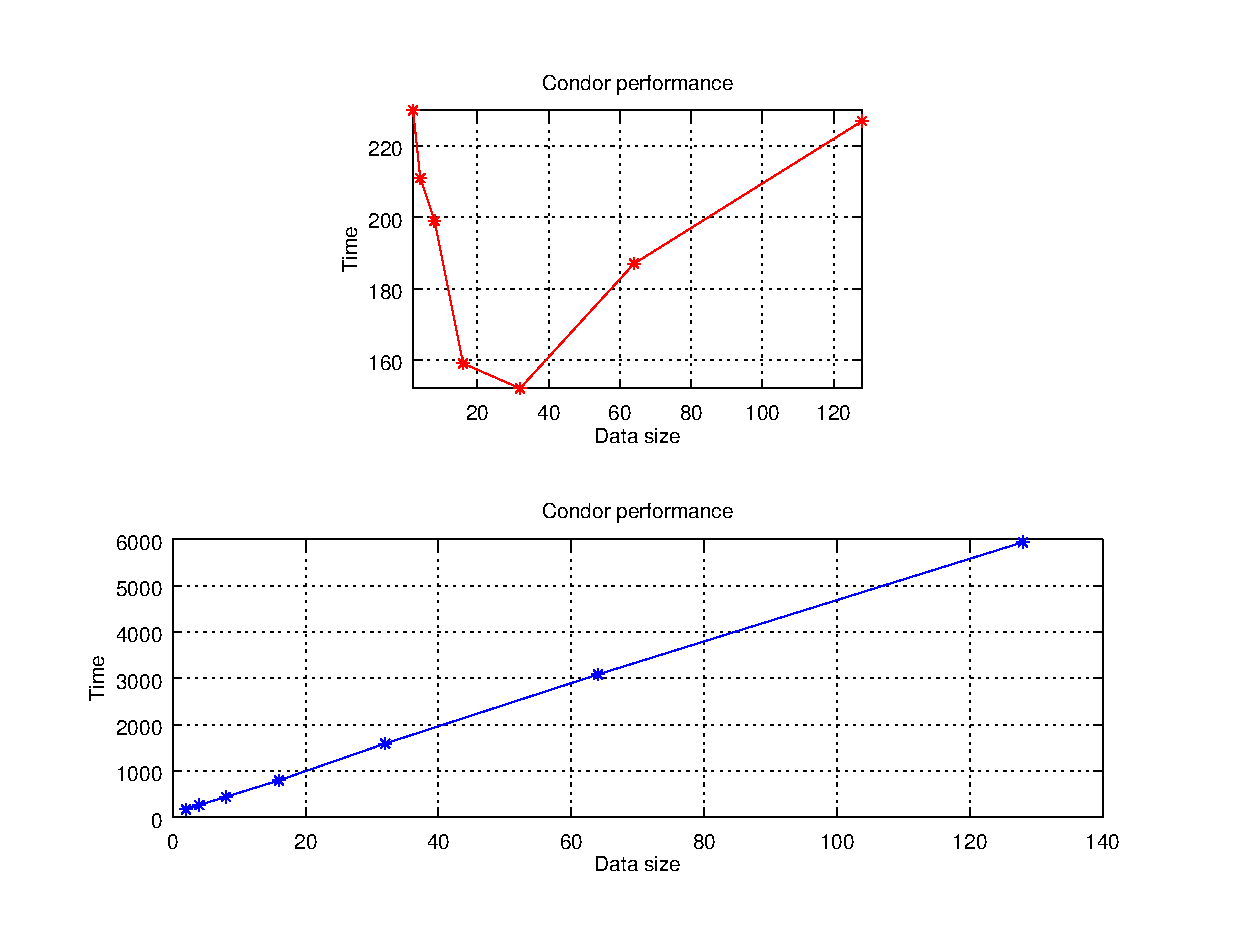
\includegraphics[width=.8\textwidth, height=1\textwidth]{OUTPUT.eps}
    \caption*{HTCondor performance}
    \label{checkerboard_lattice}
\end{figure}

\section{Limit number of cores}
The easiest way to limit the number of cores for HTCondor available on each slot (Check out section 3.5.1.12 in the manual) is by put a configuration file in the \verb+config.d+ 
folder on your compute nodes that explicitly defines the slots on that node. For example, if you had a four-core CPU and you only want condor to be able to use two,
you would use the following lines in your config file:
\begin{verbatim}
SLOT_TYPE_1 = cpus=2
NUM_SLOTS = 1
NUM_SLOTS_TYPE_1 = 1
\end{verbatim}

%\section*{HTCondor into python-Python Bindings}

%%%%%%%%%%%%%%%%%%%%
% Concluding Pages %
%%%%%%%%%%%%%%%%%%%%%%%%%%%%%%%%%%%%%%%%%%%%%%%%%%%%%%%%%%%%%%%%%%%%%%%%%%%%%%%%

% Bibliography or References, REQUIRED

% If using bibtex, create or modify the refs.bib file
% and use (uncomment) the following three lines.
%\bibliographystyle{plain}     %You may prefer \bibliographystyle{alpha}
%\addcontentsline{toc}{chapter}{\bibname}
%\bibliography{refs}         

% If using the ``thereference'' environment instead, modify the ref.tex file
% and use the following line
%\include{ref}
%\bibliography{Bibliography_HTCondor}
%\bibliography{TOOLS_Bibliography}
\bibliography{References/TOOLS_Bibliography}
\end{document}
